\documentclass[12pt]{article}

\usepackage{graphicx} % to include figures
%\graphicspath{{Figures/}} %This can be used if figures are in a folder in the Latex path
\graphicspath{{../Matlab/Figures/}} %Setting the graphicspath
\usepackage{float} % to force figure placement with [H]
\usepackage{geometry} % to set the page size and margins
\geometry{a4paper, margin=2.5cm}
\usepackage{amsmath,amsthm,amssymb} % enables \begin{subequations} and \begin{aligned}
\usepackage{matlab-prettifier} % to import MATLAB code
\usepackage[hidelinks]{hyperref} % enable hyperlinks (boxes hidden)
\usepackage{pgf} % enable pgf figures
\usepackage{siunitx} % enable SI units and notation
\usepackage{arydshln} % for partitioned matrices with dashed lines
\usepackage[numbib]{tocbibind} % give the references section a section number
\setcounter{MaxMatrixCols}{18} % if this is not done, a matrix may only contain 10 columns

%% packages for pfg plots from MATLAB's exported tex files
%% See https://github.com/matlab2tikz/matlab2tikz for details
\usepackage{pgfplots}
\pgfplotsset{compat=newest}
%% the following commands are needed for some matlab2tikz features
\usetikzlibrary{plotmarks}
\usetikzlibrary{arrows.meta}
\usepgfplotslibrary{patchplots}
\usepackage{grffile}
%% you may also want the following commands
%\pgfplotsset{plot coordinates/math parser=false}
%\newlength\figureheight
%\newlength\figurewidth

\begin{document}

\title{Assignment 7: Introduction to Constrained MPC}
\author{Charl van de Merwe, 20804157\\
Optimal Control, EBO 780}
\date{June 14, 2020}

\maketitle

\section{Assignment Overview}
The purpose of this assignment is to implement a simple constrained linear model predictive controller (MPC), without using MATLAB's MPC toolbox. A Kalman filter (KF) needs to be implemented to estimate the states and disturbances. The MPC and KF will make use of the prediction model, defined by

\renewcommand\arraystretch{1.4}
\begin{equation}
\frac{Y(s)}{U(s)} = G_C(s) =
\scalebox{1.3}{$  
\begin{bmatrix}
\frac{12.8}{16.7s+1}e^{-1s} & \frac{-18.9}{21s+1}e^{-3s}\\
\frac{6.6}{10.9s+1}e^{-7s} & \frac{-19.4}{14.4s+1}e^{-3s}
\end{bmatrix}$}. \label{eq:predModel}
\end{equation}
\renewcommand\arraystretch{1}
where $Y(s)$ is the controlled variable (CV) and $U(s)$ is the manipulated variable (MV). \\

The process model differs from the prediction model and is given by
\renewcommand\arraystretch{1.4}
\begin{equation}
G_P(s) =
\scalebox{1.3}{$  
	\begin{bmatrix}
	\frac{15.36}{16.7s+1}e^{-1s} & \frac{-18.9}{25.2s+1}e^{-3s}\\
	\frac{7.92}{10.9s+1}e^{-7s} & \frac{-19.4}{17.28s+1}e^{-3s}
	\end{bmatrix}$}. \label{eq:procModel}
\end{equation}
\renewcommand\arraystretch{1}

\section{MPC and KF Description}
\label{sec:mpcDesc}

\subsection{Problem 1: MPC Description}
\label{sec:MPCDescription}

\textbf{Problem:} Define a discrete-time linear constrained MPC by giving the objective function and optimisation problem with constraints. Further, define all the variables/parameters involved. \\

At each time instance, the MPC algorithm computes a sequence of future manipulated variables (MV) to optimize the future plant behaviour. The first input of the optimized system is then sent into the plant. The MPC algorithm is computed at every time instance, at a period equal to the sampling frequency ($ T_s $) \cite{Qin.2003}. MPC is a discrete time algorithm. The optimization problem is described mathematically as
\begin{equation}
\min_{u(k+N_C|k),...,u(k|k)} V(x(k|k),u),
\end{equation}

where $ u $ is the input to the plant, $ x $ is the plant states ($ x(k|k) $ is the initial state, measured or estimated from the plant) $N_C$ is the amount of control steps and $ V $ is the objective function to be minimized. The input and states are constrained, as defined by
%\begin{subequations}
\begin{align*}
x &\in X \\
u &\in U \\
X &\triangleq \{x \in \mathbb{R}^{N_X}|x_l \leq x \leq x_u\} \\
U &\triangleq \{u \in \mathbb{R}^{N_U}|u_l \leq u \leq u_u\}
\end{align*}
%\end{subequations}

Note that the $ |k $ term indicates that the plant behaviour is predicted from the measured states at discrete time instance $ k $. As an example, $ x(5|3) $ is the predicted states at instance $5$, propagated from the measured states at instance $3$. The objective function is
\begin{equation}
\begin{aligned}
V(x,u) = &\sum_{i=1}^{N_P} (Y_{sp}(k)-y(k+i|k))^T Q (Y_{sp}(k)-y(k+i|k)) \,+\\ &\sum_{i=1}^{N_C} \Delta u(k+i|k)^T R \,\Delta u(k+i|k), \label{eq:ObjFunc}
\end{aligned}
\end{equation}
subject to
\begin{subequations}
\begin{align}
x(k+i+1|k) &= f(x(k+i|k),u(k+i|k)) \qquad \, \forall i = 1,...,N_C\\
x(k+i+1|k) &= f(x(k+i|k),u(k+N_C|k)) \, \quad \forall i = N_C+1,...,N_P\\
y(k+i|k) &= h(x(k+i|k),u(k+i|k)) \qquad \, \forall i = 1,...,N_C\\
y(k+i|k) &= h(x(k+i|k),u(k+N_C|k)) \, \quad \forall i = N_C+1,...,N_P, 
\end{align} \label{eq:system}
\end{subequations}
where $ N_P $ is the prediction horizon, $ Y_{sp} $ is the constant setpoint or desired output of the plant, $ y $ is the predicted output, $ \Delta u $ is the input (control) step size (from one instance to another) and $Q$ and $R$ is the output and input weighing matrices. From (\ref{eq:system}) it can be seen that there are $N_C$ unique control steps, whereafter the last control step is maintained throughout the prediction horizon.

In this assignment, the future manipulated variables (MV) behaviour (or output behaviour) is specified using setpoints, as described by $ Y_{sp}(k) $ in (\ref{eq:ObjFunc}). Future MV behaviour can also be specified by using zones, reference trajectories or a funnel \cite{Qin.2003}.

\subsection{Problem 2: KF Description}
\label{sec:KFDescription}

\textbf{Problem:} Define a discrete-time Kalman filter in state-space form which can estimate both the process	states and process disturbances. \\

The Kalman filter (KF) takes the implemented CVs, $u_k$, and measurements of the MVs, $y_k$, to determine estimated states, $\hat{x}_k$. In this implementation, the Kalman filter is extended to include estimates of the process disturbances. The process disturbances, $d_k$, can be modelled as random walks. The process model is therefore defined by
\begin{subequations}
\begin{align}
x_{k+1} &= Ax_k + B(u_k+d_k) \\
d_{k+1} &= d_k + w_k \\
y_k &= Cx_k. 
\end{align} \label{eq:modelWithDisturbance}
\end{subequations}
The process model is rewritten in an augmented state space model as
\begin{subequations}
\begin{align}
z_{k+1} &= \bar{A}z_k + \bar{B}p_k \\
y_k &= \bar{C}z_k + \bar{D}p_k,
\end{align} \label{eq:augModel}
\end{subequations}
where
\begin{subequations}
\begin{align}
z_k &= \begin{bmatrix}
x_k \\ d_k
\end{bmatrix} \label{eq:augStates}\\
p_k &= \begin{bmatrix}
u_k \\ w_k
\end{bmatrix} \\
\bar{A} &= \begin{bmatrix}
A & B \\
0 & I
\end{bmatrix} \\
\bar{B} &= \begin{bmatrix}
B & 0 \\
0 & I
\end{bmatrix} \\
\bar{C} &= \begin{bmatrix}
C & 0
\end{bmatrix}. \\
\bar{D} &= 0.
\end{align} \label{eq:augModelParams}
\end{subequations}
Note that the random walk variable, $w_k$, will be set to zero in the model, but the value of the disturbance, $d_k$, will be determined and update by the Kalman filter.

The Kalman filter estimates the states in two steps. The next time step (at discrete time $k+1$) estimate, $\hat{z}_{k+1|k}$, is determined in the \textit{time update} step:
\begin{equation}
\hat{z}_{k+1|k} = \bar{A} \hat{z}_{k|k} + \bar{B} p_k, \label{eq:timeUpdate}
\end{equation}
where $ \hat{z}_{k|k} $ is the current estimate of the states determined from measurements at time $k$. The current estimate is determined in the \textit{measurement update} step:
\begin{equation}
\hat{z}_{k|k} = \hat{z}_{k|k-1} + M (y_{vk} - \bar{C} \hat{z}_k), \label{eq:measurementUpdate}
\end{equation}
where $ \hat{z}_{k|k-1} $ is the estimate of the state at time $k$, determined by the \textit{time update} step at time $k-1$, $ M $ is the Kalman gain and $ y_{vk} $ is the noisy output measurement. The \textit{time update} step can be rewritten as a state space system, by substituting (\ref{eq:measurementUpdate}) into (\ref{eq:timeUpdate}), as
\begin{subequations}
\begin{align}
\hat{z}_{k+1|k} &= A_{KF} \hat{z}_{k|k-1} B_{KF} u_{KF} \\
y_{KF} &= C_{KF} \hat{z}_{k|k-1},
\end{align} \label{eq:KF}
\end{subequations}
where 
\begin{subequations}
\begin{align}
u_{KF} &= \begin{bmatrix} p_k \\ y_{vk} \end{bmatrix} \\
A_{KF} &= \bar{A}(I-M\bar{C}) \\
B_{KF} &= \begin{bmatrix} \bar{B} & \bar{A}M \end{bmatrix} \\
C_{KF} &= I.
\end{align}
\end{subequations}
Note that the output of (\ref{eq:KF}) is $ \hat{z}_{k|k-1} $. To determine $ \hat{z}_{k|k} $, the \textit{measurement update} has to be implemented. The \textit{measurement update} step is rewritten as
\begin{equation}
\hat{z}_{k|k} = (I-M \bar{C})\hat{z}_{k|k-1} + M y_{vk}.
\end{equation}
From the output of the \textit{measurement update}, the filtered (estimated) output can be determined from
\begin{equation}
\hat{y}_{k|k} = \bar{C} \hat{z}_{k|k}. \label{eq:KFOutput}
\end{equation}

\subsection{Problem 3: Process Model}

\textbf{Problem:} Based on the specifications above, give the process model $G_P(s)$ in continuous LTI format. \\

The continuous process model is given in (\ref{eq:procModel}).

\section{System Description in Discrete Time}

\subsection{Problem 4: Discrete State-Space Prediction Model}

\textbf{Problem:} Create a discrete state-space prediction based on the continuous model, by discretizing it with a sampling time of 1 second. \\

The continuous model in (\ref{eq:predModel}) is converted to a discrete-time model using MATLAB's \textit{c2d} function, with a sampling time of $T_s = 1 \,s$. The discrete-time model is converted to a state-space model by using MATLAB's \textit{ss} function. The time-delays are then mapped to discrete-time state by using the \textit{absorbDelay} function, as seen in Section \ref{code:Setup}. The resulting model is
\begin{subequations}
\begin{align}
x_{k+1} &= Ax_k + Bu_k \\
y_k &= Cx_k + Du_k.
\end{align} \label{eq:PredModel}
\end{subequations}
with the $A$, $B$ and $C$ matrices corresponding to the matrices in (\ref{eq:modelWithDisturbance}) and (\ref{eq:augModelParams}). These matrices are
\begin{subequations}
\begin{equation}
A = \begin{bmatrix}
0.9419	&0	&0	&0&	0&	0&	0&	0&	0&	0	&1&	0&	0&	0\\
0&	0.9123&	0&	0&	0&	0&	0&	0&	0&	0&	1&	0&	0&	0\\
0&	0&	0.9535&	0&	0&	0&	0&	0&	0&	0&	0&	1&	0&	0\\
0&	0&	0&	0.9329&	0&	0&	0&	0&	0&	0&	0&	1&	0&	0\\
0&	0&	0&	0&	0&	1&	0&	0&	0&	0&	0&	0&	0&	0\\
0&	0&	0&	0&	0&	0	&1	&0&	0&	0&	0&	0&	0&	0\\
0&	0&	0&	0&	0&	0&	0&	1&	0&	0&	0&	0&	0&	0\\
0&	0&	0&	0&	0&	0&	0&	0&	1&	0&	0&	0&	0&	0\\
0&	0&	0&	0&	0&	0&	0&	0&	0&	1&	0&	0&	0&	0\\
0&	0.5786&	0&	0&	0&	0&	0&	0&	0&	0&	0&	0&	0&	0\\
0&	0&	0&	0&	0&	0&	0&	0&	0&	0&	0&	0&	0&	0\\
0&	0&	0&	0&	0&	0&	0&	0&	0&	0&	0&	0&	1&	0\\
0&	0&	0&	0&	0&	0&	0&	0&	0&	0&	0&	0&	0&	1\\
0&	0&	0&	0&	0&	0&	0&	0&	0&	0&	0&	0&	0&	0
\end{bmatrix}
\end{equation}
\begin{align}
B &= \begin{bmatrix}
0&	0\\
0&	0\\
0&	0\\
0&	0\\
0&	0\\
0&	0\\
0&	0\\
0&	0\\
0&	0\\
0&	0\\
1&	0\\
0&	0\\
0&	0\\
0&	1
\end{bmatrix} \\
C &= \begin{bmatrix}
0.7440&	0&	-0.8789&	0&	0&	0&	0&	0&	0&	0&	0&	0&	0&	0 \\
0&	0&	0&	-1.3015&	1&	0&	0&	0&	0&	0&	0&	0&	0&	0
\end{bmatrix} \\
D &= \begin{bmatrix}
0&	0\\
0&	0
\end{bmatrix}
\end{align}
\end{subequations}

\subsection{Problem 5: KF Model}

\textbf{Problem:} Create a discrete state-space model for the Kalman filter, based on your discrete-time model for the MPC. The KF should also estimate the process disturbances. \\

The answer to this problem is included in Section \ref{sec:KFDescription} (Problem 2). This is implemented in code, as can be seen in Section \ref{code:Setup}.

\subsection{Problem 6: KF Gain}

\textbf{Problem:} Create a discrete-time linear KF using the MATLAB command “kalman”, based on the state-space KF model. \\

The augmented state-space prediction model defined in (\ref{eq:augModel}) and (\ref{eq:augModelParams}) are used in MATLAB's \textit{kalman} function to determine the Kalman gain, as can be seen in Section \ref{code:Setup}. In addition to the process noise, $w_k$, measurements of the output includes noise, $v_y$. The augmented process model for the Kalman filter is therefore given by (note that $\bar{D}=0$)
\begin{subequations}
\begin{align}
z_{k+1} &= \bar{A}z_k + \bar{B} \begin{bmatrix} u_k \\ w_k \end{bmatrix} \\
y_k &= \bar{C}z_k + v_k,
\end{align} \label{eq:augModelwithNoise}
\end{subequations}
where $w_k$ is the process noise with a covariance of $E(w_k w_k^T)=Q_{KF}$ and $v_k$ is the measurement noise with a covariance of $E(v_k v_k^T)=R_{KF}$. It may not always be possible to physically measure the noise covariances. The $Q_{KF}$ and $R_{KF}$ matrices are chosen based on prior knowledge of the process and measurement noise and tuned to produce the best possible control. The absolute value of $Q_{KF}$, $R_{KF}$ or elements within the matrices do not matter, but their values with respect to each other do.

In the simulation done in this assignment, there is no reason to expect that the noise will be greater on one of the inputs or outputs than of the other. Therefore $Q_{KF11}=Q_{KF22}$ and $R_{KF11}=R_{KF22}$ where chosen. The output noise in this simulation contributes more to the disturbance of the system than the input noise, therefore  $R_{KF}=50 Q_{KF}$ was chosen. The chosen noise covariance matrices are
\begin{subequations}
\begin{align}
Q_{KF} &= \begin{bmatrix}
1 & 0 \\
0 & 1
\end{bmatrix} \\
R_{KF} &= \begin{bmatrix}
50 & 0 \\
0 & 50
\end{bmatrix}
\end{align} \label{eq:NoiseCovarianceMatrices}
\end{subequations}

Based on the augmented process matrices defined in (\ref{eq:augModelParams}) and the noise covariance matrices in (\ref{eq:NoiseCovarianceMatrices}), the Kalman gain is
\begin{equation}
M = \begin{bmatrix}
0.4218&   -0.2423 \\
0.3965&   -0.2233\\
-0.0608&   -0.3204\\
-0.0618&  -0.3101\\
0.0210&   -0.0227\\
0.0405&   -0.0335\\
0.0668&   -0.0489\\
0.0999&   -0.0677\\
0.1394&   -0.0883\\
0.1836&   -0.1092\\
0.1070&   -0.0511\\
-0.0348&   -0.0989\\
-0.0348&   -0.0989\\
-0.0348&   -0.0989\\
0.1070&   -0.0511\\
-0.0348&   -0.0989
\end{bmatrix}
\end{equation}

\section{Simulink Model}
\label{sec:SimulinkModel}

The complete Simulink model can be seen in Figure \ref{fig:FullModel}. The plant, $G_p$ is as defined in (\ref{eq:procModel}). The MPC block is implemented by using a level-2 MATLAB s-function block, as seen in Figure \ref{fig:FullModel}. This block allows the use of MATLAB language to create a custom block. The MPC block reads the estimated state and filtered disturbances. The MPC algorithm is implemented within the MPC block, so that the output of the block is the optimal control steps for the plant. The implementation of the code for this block can be seen in Section \ref{code:mpcL2}.

The state and disturbance estimates are done by the \textit{Kalman Filter} block, as can be seen in Figure \ref{fig:KalmanFilter}. The \textit{Kalman Filter} block implements (\ref{eq:KF}) to (\ref{eq:KFOutput}), to determine a current estimate of the states (including disturbance) and output based on the implemented input/control, measured output and previous predicted states ($x_{k|k-1}$).

The disturbance estimate is filtered by the \textit{State Disturbance Filter} block seen in Figure \ref{fig:StateDisturbanceFilter}. This filter is explained in Section \ref{sec:DisturbanceFilter}.

The sampling time for the discrete plant and for the MPC block is 1 second. The Simulink \textit{solver options} are therefore set to use \textit{Runge-Kutta} with a \textit{fixed-step size} of 1 second.

\begin{figure}[H]
	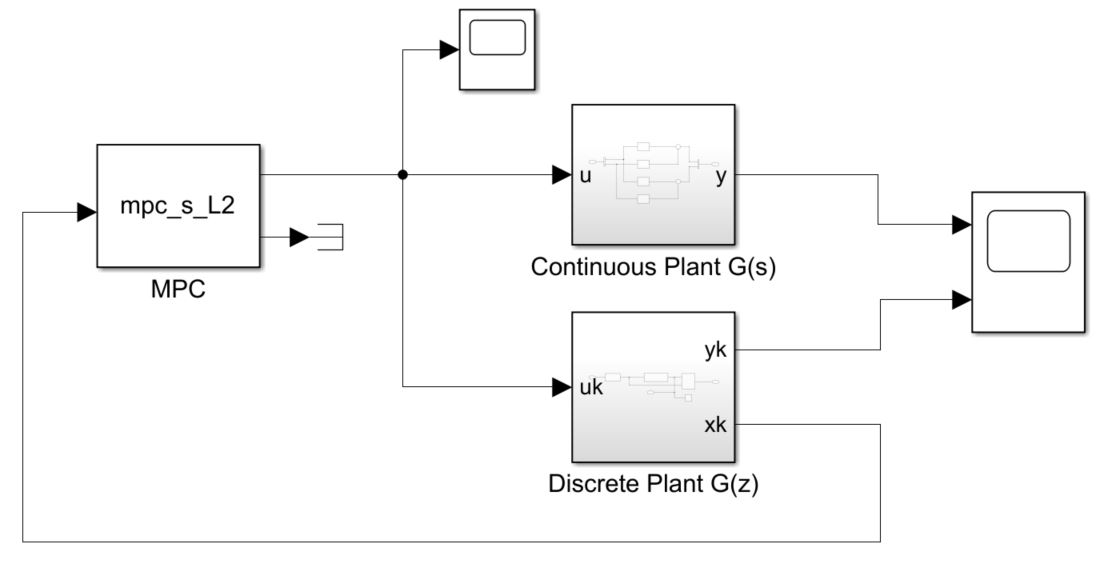
\includegraphics[width=17cm]{FullModel.jpg}
	\centering
	\caption{Simulink Model}
	\label{fig:FullModel}
\end{figure}

\begin{figure}[H]
	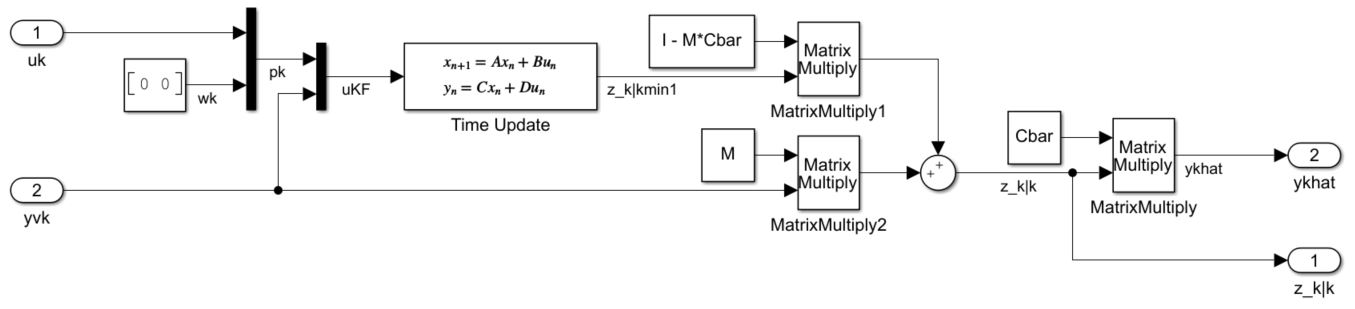
\includegraphics[width=17cm]{KalmanFilter.jpg}
	\centering
	\caption{Kalman Filter Block}
	\label{fig:KalmanFilter}
\end{figure}

\begin{figure}[H]
	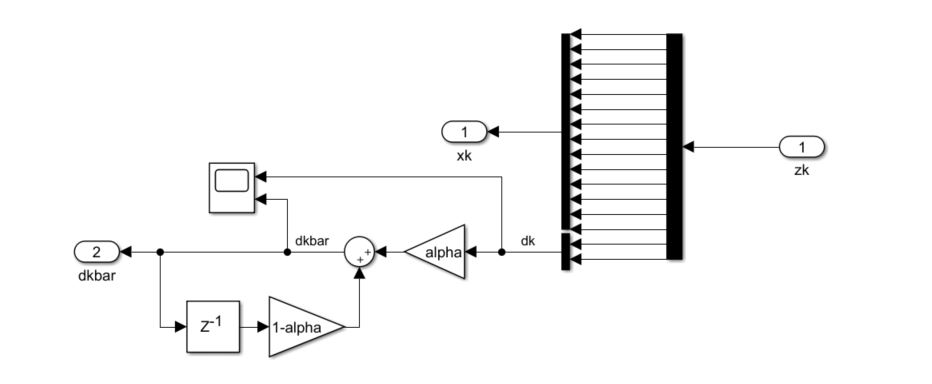
\includegraphics[width=15cm]{StateDisturbanceFilter.jpg}
	\centering
	\caption{State Disturbance Filter Block}
	\label{fig:StateDisturbanceFilter}
\end{figure}

\section{MPC Controller}

\subsection{Problem 7: MPC Constraints}

\textbf{Problem:} Code the MATLAB function “constraints” that enforces constraints on the inputs. This function will be included as part of the optimization function in the MPC. The constraints for $G_C(s)$ on the manipulated variable (MV) 1 are $(-\infty, 1]$ and on MV 2 are $[-4, \infty)$. \\

Constrained MPC finds the optimal controlled variables (CV) for which the objective function
\begin{equation}
\min_{u(k+N_C|k),...,u(k|k)} V(x(k|k),u),
\end{equation}
is minimized such that
\begin{subequations}
\begin{align}
c(x,u) &\leq 0 \\
c_{eq}(x,u) &= 0,
\end{align}
\end{subequations}
where linear and non-linear inequality and equality constraints are captured in $c(x,u)$ and $c_{eq}(x,u)$. The inequality constraints defined in the problem can be formulated as
\begin{equation}
c(u) = \begin{bmatrix}
u_1 - 1 \\
-u_2 - 4
\end{bmatrix} \leq 0. \label{eq:constraints}
\end{equation}

As stated in Section \ref{sec:MPCDescription}, there are $N_C$ unique control steps in the MPC prediction. The constraints needs to be imposed on each of these control steps. The inequality constraints vector implemented is therefore
\begin{equation}
c(u) = \begin{bmatrix}
u_1(k|k) - 1 \\
\vdots \\
u_1(k+N_C|k) - 1 \\
-u_2(k|k) - 4 \\
\vdots \\
-u_2(k+N_C|k) - 4
\end{bmatrix}.
\end{equation}

The constraints are defined in the \textit{getConstraints} function, as can be seen in Section \ref{code:getConstraints}. These constraints are passed to the \textit{fmincon} function in the \textit{nonlcon} argument, as can be seen in Section \ref{code:mpc}.

\subsection{Problem 8: MPC Algorithm Description}

\textbf{Problem:} Code the Matlab function \textit{ObjFunc} that calculates the objective value that will be optimized by \textit{fmincon}. Your MPC controller must implement blocking to allow for a smooth closed-loop MV trajectory. The function “\textit{ObjFunc}” should use the disturbance estimate from your KF as part of the predictions. Show the algorithm “\textit{ObjFunc}” uses to calculates the predictions for the MPC. \\

As mentioned in Section \ref{sec:mpcDesc}, the MPC algorithm computes the optimal input steps to produce the desired future output (or manipulated variables). The MPC algorithm can be summarized in the following steps:
\begin{enumerate}
	\item Guess the optimal future inputs.
	\item Predict the future output, based on the guessed inputs, from (\ref{eq:PredModel}). 
	\item Compute the quadratic penalty (cost) due to the difference of the output to the setpoints and the difference between input steps, as described by the objective function defined in (\ref{eq:ObjFunc}).
	\item Repeat step 1 to 3 to find the optimal input steps.
\end{enumerate}

These steps are followed within MATLAB's \textit{fmincon} function. This function will numerically compute the optimal input steps, within the constraints defined in the constraints function, to minimize the objective function.

The implementation of the MPC algorithm can be seen in Section \ref{code:mpc}. The constraints are defined in the \textit{getConstraints} function as seen in Section \ref{code:getConstraints}. The computation of the objective function can be seen in Section \ref{code:objectiveFunc}. The implementation of the output prediction can be seen in Section \ref{code:prediction}.

The output and input weighing matrices, $Q$ and $R$, as seen in the objective function in (\ref{eq:ObjFunc}), were chosen to be
\begin{subequations}
\begin{align}
Q &=
\begin{bmatrix}
1 & 0 \\
0 & 1.4
\end{bmatrix} \\[0.5ex]
R &=
\begin{bmatrix}
0.01 & 0 \\
0 & 0.04
\end{bmatrix}.
\end{align}
\end{subequations}

\subsection{Testing the MPC Algorithm}

A script to test the MPC algorithm, for the plant in (\ref{eq:predModel}) starting from rest with a [5,-5] setpoint, can be seen in Section \ref{code:TestMPC}. The result of this test can be seen in Figure \ref{fig:TestMPC}.

The \textit{fmincon} function computes the optimal input steps for this test script to be ($N_C=3$ was chosen):
\begin{align}
U^* &= \begin{bmatrix}
u^*_1(k|k) & u^*_1(k+1|k) & u^*_1(k+3|k) \\
u^*_2(k|k) & u^*_2(k+1|k) & u^*_2(k+3|k)
\end{bmatrix} \\[0.5ex]
&= \begin{bmatrix}
1.0000&    0.9390&    0.5442 \\
2.0758&    2.1836&    1.7889
\end{bmatrix}. \nonumber
\end{align}
The first two input steps are maintained for six samples each, as specified by the blocking parameter $N_B=6$, and the last input step is maintained for the full duration of the prediction horizon. None of the input values exceed the constraints defined in (\ref{eq:constraints}). The plot is limited to 60 samples, but the chosen prediction horizon is $N_P=100$.

These parameters are only relevant to the prediction simulation. In each time instance of the physical system, the MPC algorithm is repeated to compute the optimal control input. The control input sent into the plant is not maintained as it is done in the prediction simulation (blocking implementation).

\begin{figure}[H]
	% This file was created by matlab2tikz.
%
%The latest updates can be retrieved from
%  http://www.mathworks.com/matlabcentral/fileexchange/22022-matlab2tikz-matlab2tikz
%where you can also make suggestions and rate matlab2tikz.
%
\definecolor{mycolor1}{rgb}{0.00000,0.44700,0.74100}%
\definecolor{mycolor2}{rgb}{0.85000,0.32500,0.09800}%
\definecolor{mycolor3}{rgb}{0.92900,0.69400,0.12500}%
\definecolor{mycolor4}{rgb}{0.49400,0.18400,0.55600}%
%
\begin{tikzpicture}

\begin{axis}[%
width=4.844in,
height=3.396in,
at={(0.813in,0.458in)},
scale only axis,
xmin=0,
xmax=60,
xlabel style={font=\color{white!15!black}},
xlabel={Samples from system discrete time k},
ymin=-6,
ymax=6,
axis background/.style={fill=white},
title style={font=\bfseries},
title={MPC Optimized Input and Predicted Output},
legend style={at={(0.97,0.5)}, anchor=east, legend cell align=left, align=left, draw=white!15!black}
]
\addplot[const plot, color=mycolor1] table[row sep=crcr] {%
0	0\\
1	0\\
2	1.48794043661385\\
3	2.88939779705764\\
4	3.26387369107736\\
5	3.60559739570094\\
6	3.91698346838632\\
7	4.20028236706281\\
8	4.4121790166945\\
9	4.60267848197739\\
10	4.67871058944432\\
11	4.74096649138508\\
12	4.79068202744093\\
13	4.82900097209096\\
14	4.56328524012395\\
15	4.30527943072257\\
16	4.40181912724793\\
17	4.48974722174962\\
18	4.5697037739367\\
19	4.64228515294933\\
20	4.70804687851057\\
21	4.76750628291091\\
22	4.82114500489206\\
23	4.86941132582231\\
24	4.91272235792336\\
25	4.95146609371335\\
26	4.98600332527193\\
27	5.01666944140799\\
28	5.0437761103169\\
29	5.06761285485067\\
30	5.0884485270882\\
31	5.10653268848393\\
32	5.122096901488\\
33	5.13535593817\\
34	5.14650891103882\\
35	5.155740330932\\
36	5.16322109654864\\
37	5.16910941991824\\
38	5.17355169183375\\
39	5.17668329102856\\
40	5.17862934064429\\
41	5.17950541531669\\
42	5.17941820200204\\
43	5.17846611747238\\
44	5.17673988522738\\
45	5.17432307439957\\
46	5.17129260307035\\
47	5.1677192082635\\
48	5.16366788474237\\
49	5.15919829460419\\
50	5.15436514954099\\
51	5.14921856751972\\
52	5.14380440552483\\
53	5.13816456990372\\
54	5.13233730575899\\
55	5.1263574667409\\
56	5.12025676650859\\
57	5.11406401304856\\
58	5.10780532696456\\
59	5.10150434478236\\
60	5.09518240824725\\
61	5.08885874053045\\
62	5.0825506102022\\
63	5.07627348377534\\
64	5.07004116757198\\
65	5.06386593961797\\
66	5.05775867222519\\
67	5.05172894587932\\
68	5.04578515501148\\
69	5.03993460619517\\
70	5.03418360927499\\
71	5.02853756190133\\
72	5.02300102791454\\
73	5.01757780999375\\
74	5.01227101695835\\
75	5.0070831260854\\
76	5.00201604078242\\
77	4.99707114393312\\
78	4.99224934721287\\
79	4.9875511366515\\
80	4.98297661470254\\
81	4.97852553906155\\
82	4.97419735845973\\
83	4.96999124564446\\
84	4.96590612774428\\
85	4.96194071420297\\
86	4.9580935224548\\
87	4.95436290150182\\
88	4.9507470535435\\
89	4.94724405379845\\
90	4.94385186864911\\
91	4.94056837223132\\
92	4.93739136158226\\
93	4.93431857045297\\
94	4.93134768188398\\
95	4.92847633963642\\
96	4.92570215856404\\
97	4.92302273400638\\
98	4.92043565027715\\
99	4.91793848831737\\
100	4.91552883257756\\
101	4.91320427718895\\
102	4.91096243147961\\
103	4.90880092488721\\
104	4.90671741131678\\
105	4.90470957298812\\
106	4.90277512381456\\
107	4.9009118123517\\
108	4.89911742435196\\
109	4.89738978495819\\
110	4.89572676056733\\
111	4.89412626039248\\
112	4.89258623775015\\
113	4.89110469109706\\
114	4.88967966483921\\
115	4.88830924993441\\
116	4.88699158430742\\
117	4.88572485309599\\
118	4.88450728874408\\
};
\addlegendentry{$y_1^*(k|k)$}

\addplot[const plot, color=mycolor2] table[row sep=crcr] {%
0	0\\
1	0\\
2	0\\
3	0\\
4	-1.4001567514518\\
5	-2.70637973129799\\
6	-3.92497077212905\\
7	-5.06180892894096\\
8	-4.96526000697591\\
9	-4.89899316528328\\
10	-4.99917770497963\\
11	-5.11245530488457\\
12	-5.23621065031048\\
13	-5.36815614282112\\
14	-5.54161193833568\\
15	-5.71643227743428\\
16	-5.37765223875477\\
17	-5.07242213809773\\
18	-4.79754252696954\\
19	-4.55011176065993\\
20	-4.55589582469796\\
21	-4.56409084085963\\
22	-4.57428970186057\\
23	-4.58613412093886\\
24	-4.59930947113619\\
25	-4.61354013608082\\
26	-4.62858532346792\\
27	-4.64423529697777\\
28	-4.66030798649968\\
29	-4.67664594027957\\
30	-4.69311358601403\\
31	-4.70959477100633\\
32	-4.72599055430724\\
33	-4.74221722631272\\
34	-4.75820453360421\\
35	-4.77389408891719\\
36	-4.78923794802937\\
37	-4.80419733708885\\
38	-4.8187415154712\\
39	-4.83284676067697\\
40	-4.84649546307182\\
41	-4.85967531944078\\
42	-4.87237861538926\\
43	-4.88460158758463\\
44	-4.89634385770318\\
45	-4.90760793073695\\
46	-4.91839875102966\\
47	-4.92872331005882\\
48	-4.93859030056711\\
49	-4.94800981217742\\
50	-4.95699306410584\\
51	-4.96555217102197\\
52	-4.97369993849887\\
53	-4.9814496848507\\
54	-4.98881508647759\\
55	-4.99581004412766\\
56	-5.00244856774902\\
57	-5.00874467784127\\
58	-5.01471232143058\\
59	-5.02036530098542\\
60	-5.02571721476457\\
61	-5.03078140724636\\
62	-5.03557092842984\\
63	-5.0400985009265\\
64	-5.04437649387635\\
65	-5.04841690282582\\
66	-5.05223133479821\\
67	-5.05583099787164\\
68	-5.05922669465467\\
69	-5.06242881911768\\
70	-5.06544735629926\\
71	-5.06829188446111\\
72	-5.07097157931449\\
73	-5.07349521998479\\
74	-5.07587119642053\\
75	-5.07810751798812\\
76	-5.08021182302537\\
77	-5.08219138915472\\
78	-5.08405314418259\\
79	-5.08580367743344\\
80	-5.08744925138707\\
81	-5.08899581350577\\
82	-5.09044900815333\\
83	-5.09181418852226\\
84	-5.09309642849774\\
85	-5.09430053439809\\
86	-5.09543105654095\\
87	-5.09649230059321\\
88	-5.09748833867004\\
89	-5.09842302015521\\
90	-5.09929998222045\\
91	-5.10012266002679\\
92	-5.10089429659539\\
93	-5.10161795233878\\
94	-5.10229651424715\\
95	-5.10293270472705\\
96	-5.10352909009213\\
97	-5.1040880887079\\
98	-5.10461197879407\\
99	-5.10510290588959\\
100	-5.10556288998662\\
101	-5.10599383234089\\
102	-5.10639752196648\\
103	-5.10677564182378\\
104	-5.10712977471006\\
105	-5.10746140886206\\
106	-5.10777194328077\\
107	-5.10806269278823\\
108	-5.10833489282658\\
109	-5.10858970400963\\
110	-5.10882821643675\\
111	-5.10905145377941\\
112	-5.10926037714993\\
113	-5.1094558887622\\
114	-5.10963883539393\\
115	-5.10981001165935\\
116	-5.10997016310159\\
117	-5.11011998911326\\
118	-5.11026014569366\\
};
\addlegendentry{$y_2^*(k|k)$}

\addplot[const plot, color=mycolor3] table[row sep=crcr] {%
0	0.999999993637481\\
1	0.999999993637481\\
2	0.999999993637481\\
3	0.999999993637481\\
4	0.999999993637481\\
5	0.999999993637481\\
6	0.938959813609464\\
7	0.938959813609464\\
8	0.938959813609464\\
9	0.938959813609464\\
10	0.938959813609464\\
11	0.938959813609464\\
12	0.54419120806217\\
13	0.54419120806217\\
14	0.54419120806217\\
15	0.54419120806217\\
16	0.54419120806217\\
17	0.54419120806217\\
18	0.54419120806217\\
19	0.54419120806217\\
20	0.54419120806217\\
21	0.54419120806217\\
22	0.54419120806217\\
23	0.54419120806217\\
24	0.54419120806217\\
25	0.54419120806217\\
26	0.54419120806217\\
27	0.54419120806217\\
28	0.54419120806217\\
29	0.54419120806217\\
30	0.54419120806217\\
31	0.54419120806217\\
32	0.54419120806217\\
33	0.54419120806217\\
34	0.54419120806217\\
35	0.54419120806217\\
36	0.54419120806217\\
37	0.54419120806217\\
38	0.54419120806217\\
39	0.54419120806217\\
40	0.54419120806217\\
41	0.54419120806217\\
42	0.54419120806217\\
43	0.54419120806217\\
44	0.54419120806217\\
45	0.54419120806217\\
46	0.54419120806217\\
47	0.54419120806217\\
48	0.54419120806217\\
49	0.54419120806217\\
50	0.54419120806217\\
51	0.54419120806217\\
52	0.54419120806217\\
53	0.54419120806217\\
54	0.54419120806217\\
55	0.54419120806217\\
56	0.54419120806217\\
57	0.54419120806217\\
58	0.54419120806217\\
59	0.54419120806217\\
60	0.54419120806217\\
61	0.54419120806217\\
62	0.54419120806217\\
63	0.54419120806217\\
64	0.54419120806217\\
65	0.54419120806217\\
66	0.54419120806217\\
67	0.54419120806217\\
68	0.54419120806217\\
69	0.54419120806217\\
70	0.54419120806217\\
71	0.54419120806217\\
72	0.54419120806217\\
73	0.54419120806217\\
74	0.54419120806217\\
75	0.54419120806217\\
76	0.54419120806217\\
77	0.54419120806217\\
78	0.54419120806217\\
79	0.54419120806217\\
80	0.54419120806217\\
81	0.54419120806217\\
82	0.54419120806217\\
83	0.54419120806217\\
84	0.54419120806217\\
85	0.54419120806217\\
86	0.54419120806217\\
87	0.54419120806217\\
88	0.54419120806217\\
89	0.54419120806217\\
90	0.54419120806217\\
91	0.54419120806217\\
92	0.54419120806217\\
93	0.54419120806217\\
94	0.54419120806217\\
95	0.54419120806217\\
96	0.54419120806217\\
97	0.54419120806217\\
98	0.54419120806217\\
99	0.54419120806217\\
100	0.54419120806217\\
101	0.54419120806217\\
102	0.54419120806217\\
103	0.54419120806217\\
104	0.54419120806217\\
105	0.54419120806217\\
106	0.54419120806217\\
107	0.54419120806217\\
108	0.54419120806217\\
109	0.54419120806217\\
110	0.54419120806217\\
111	0.54419120806217\\
112	0.54419120806217\\
113	0.54419120806217\\
114	0.54419120806217\\
115	0.54419120806217\\
116	0.54419120806217\\
117	0.54419120806217\\
118	0.54419120806217\\
};
\addlegendentry{$u_1^*(k|k)$}

\addplot[const plot, color=mycolor4] table[row sep=crcr] {%
0	2.07579575795987\\
1	2.07579575795987\\
2	2.07579575795987\\
3	2.07579575795987\\
4	2.07579575795987\\
5	2.07579575795987\\
6	2.18358427038044\\
7	2.18358427038044\\
8	2.18358427038044\\
9	2.18358427038044\\
10	2.18358427038044\\
11	2.18358427038044\\
12	1.78886239090085\\
13	1.78886239090085\\
14	1.78886239090085\\
15	1.78886239090085\\
16	1.78886239090085\\
17	1.78886239090085\\
18	1.78886239090085\\
19	1.78886239090085\\
20	1.78886239090085\\
21	1.78886239090085\\
22	1.78886239090085\\
23	1.78886239090085\\
24	1.78886239090085\\
25	1.78886239090085\\
26	1.78886239090085\\
27	1.78886239090085\\
28	1.78886239090085\\
29	1.78886239090085\\
30	1.78886239090085\\
31	1.78886239090085\\
32	1.78886239090085\\
33	1.78886239090085\\
34	1.78886239090085\\
35	1.78886239090085\\
36	1.78886239090085\\
37	1.78886239090085\\
38	1.78886239090085\\
39	1.78886239090085\\
40	1.78886239090085\\
41	1.78886239090085\\
42	1.78886239090085\\
43	1.78886239090085\\
44	1.78886239090085\\
45	1.78886239090085\\
46	1.78886239090085\\
47	1.78886239090085\\
48	1.78886239090085\\
49	1.78886239090085\\
50	1.78886239090085\\
51	1.78886239090085\\
52	1.78886239090085\\
53	1.78886239090085\\
54	1.78886239090085\\
55	1.78886239090085\\
56	1.78886239090085\\
57	1.78886239090085\\
58	1.78886239090085\\
59	1.78886239090085\\
60	1.78886239090085\\
61	1.78886239090085\\
62	1.78886239090085\\
63	1.78886239090085\\
64	1.78886239090085\\
65	1.78886239090085\\
66	1.78886239090085\\
67	1.78886239090085\\
68	1.78886239090085\\
69	1.78886239090085\\
70	1.78886239090085\\
71	1.78886239090085\\
72	1.78886239090085\\
73	1.78886239090085\\
74	1.78886239090085\\
75	1.78886239090085\\
76	1.78886239090085\\
77	1.78886239090085\\
78	1.78886239090085\\
79	1.78886239090085\\
80	1.78886239090085\\
81	1.78886239090085\\
82	1.78886239090085\\
83	1.78886239090085\\
84	1.78886239090085\\
85	1.78886239090085\\
86	1.78886239090085\\
87	1.78886239090085\\
88	1.78886239090085\\
89	1.78886239090085\\
90	1.78886239090085\\
91	1.78886239090085\\
92	1.78886239090085\\
93	1.78886239090085\\
94	1.78886239090085\\
95	1.78886239090085\\
96	1.78886239090085\\
97	1.78886239090085\\
98	1.78886239090085\\
99	1.78886239090085\\
100	1.78886239090085\\
101	1.78886239090085\\
102	1.78886239090085\\
103	1.78886239090085\\
104	1.78886239090085\\
105	1.78886239090085\\
106	1.78886239090085\\
107	1.78886239090085\\
108	1.78886239090085\\
109	1.78886239090085\\
110	1.78886239090085\\
111	1.78886239090085\\
112	1.78886239090085\\
113	1.78886239090085\\
114	1.78886239090085\\
115	1.78886239090085\\
116	1.78886239090085\\
117	1.78886239090085\\
118	1.78886239090085\\
};
\addlegendentry{$u_2^*(k|k)$}

\end{axis}
\end{tikzpicture}%
	\centering
	\caption{MPC Test Result}
	\label{fig:TestMPC}
\end{figure}

\section{Simulation}

\subsection{Problem 9: Disturbance Filter}
\label{sec:DisturbanceFilter}

\textbf{Problem:} Add an extra input to your s-function m-file to read in your disturbance estimate from your KF. Exponentially filter the disturbance estimate to remove unwanted noise from the estimate. Add the filtered disturbance estimate to the MV values of your prediction model in such a way that the MV constraints will still be honoured by your MPC controller. \\

The Kalman filter includes process disturbances, $d_k$, as a state, as can be seen in (\ref{eq:augStates}). The KF therefore estimates the process disturbance. An exponential filter is used to filter the estimated disturbance. The filter is described by 
\begin{equation}
\bar{d}_k = \alpha d_k + (1-\alpha) \bar{d}_{k-1},
\end{equation}
where $ \bar{d}_k $ is the filtered disturbance, $ \bar{d}_{k-1} $ is the previous filtered value, $d_k$ is the KF estimate of the disturbance and $ \alpha $ is a fraction between 0 and 1 that controls the amount of filtering. The implementation of the filter can be seen in Figure \ref{fig:StateDisturbanceFilter}. The filter with $ \alpha = 0.3 $ produces the result in Figure \ref{fig:Disturbance}.

\begin{figure}[H]
	% This file was created by matlab2tikz.
%
%The latest updates can be retrieved from
%  http://www.mathworks.com/matlabcentral/fileexchange/22022-matlab2tikz-matlab2tikz
%where you can also make suggestions and rate matlab2tikz.
%
\definecolor{mycolor1}{rgb}{0.00000,0.44700,0.74100}%
\definecolor{mycolor2}{rgb}{0.85000,0.32500,0.09800}%
\definecolor{mycolor3}{rgb}{0.92900,0.69400,0.12500}%
\definecolor{mycolor4}{rgb}{0.49400,0.18400,0.55600}%
%
\begin{tikzpicture}

\begin{axis}[%
width=4.844in,
height=3.396in,
at={(0.812in,0.458in)},
scale only axis,
xmin=0,
xmax=250,
xlabel style={font=\color{white!15!black}},
xlabel={Simulink Discrete Time k},
ymin=-1.5,
ymax=2,
axis background/.style={fill=white},
title style={font=\bfseries},
title={Disturbance Filter},
legend style={at={(0.97,0.5)}, anchor=east, legend cell align=left, align=left, draw=white!15!black}
]
\addplot[const plot, color=mycolor1] table[row sep=crcr] {%
0	0.0402443982728804\\
1	0.0516087895943623\\
2	0.033160765721624\\
3	-6.81871096275162e-05\\
4	0.00917286832210533\\
5	-0.0245927893943813\\
6	-0.0183460505313448\\
7	-0.0357562071172709\\
8	-0.0201533450059572\\
9	0.0016770938011191\\
10	-0.0149741377819959\\
11	0.0224194294288643\\
12	0.143532490403644\\
13	0.267074618749505\\
14	0.44460346304\\
15	0.625617892636848\\
16	0.799294543313329\\
17	0.950748315821498\\
18	1.01873379959261\\
19	1.06645060211275\\
20	1.10556045779324\\
21	1.05569035313019\\
22	1.02561556880565\\
23	0.998475101789488\\
24	1.01712492673949\\
25	1.0060125769513\\
26	1.01290553094714\\
27	1.02913865065397\\
28	1.03565767902884\\
29	1.02833540523012\\
30	0.99720246680929\\
31	0.979633966889847\\
32	0.983768942641414\\
33	0.964152467264325\\
34	0.93819441269442\\
35	0.948618301079191\\
36	0.919606501995453\\
37	0.95332693691142\\
38	0.96928192511388\\
39	0.978928243627886\\
40	1.00633371245949\\
41	0.998797080416802\\
42	0.975879409488619\\
43	0.983554471880816\\
44	0.96531161950022\\
45	0.979039702035721\\
46	0.964918753342398\\
47	0.953989956684329\\
48	0.993971617519777\\
49	0.990617972481663\\
50	0.993236907298728\\
51	1.00825100189793\\
52	0.981110976125779\\
53	1.00632239217564\\
54	0.992411622970056\\
55	0.999648995295923\\
56	0.97693333868119\\
57	0.972342357522569\\
58	0.983542711204852\\
59	0.992692666818202\\
60	0.98710809770353\\
61	1.01048272760193\\
62	1.03077546063372\\
63	1.02228840330555\\
64	0.994285250686749\\
65	0.959487923428882\\
66	0.993315086127715\\
67	0.961532078809453\\
68	1.0012570914271\\
69	0.988950999187268\\
70	1.01959418396099\\
71	1.02581962085005\\
72	1.01050220891474\\
73	0.984186751371382\\
74	0.98734749896504\\
75	1.00520745477886\\
76	1.01615211221514\\
77	0.979800111924005\\
78	0.982681258630785\\
79	0.978608236494294\\
80	1.13850801153595\\
81	1.26707672314845\\
82	1.35742316931231\\
83	1.40349975889518\\
84	1.40492054852632\\
85	1.41705121064604\\
86	1.38161793625569\\
87	1.31310303741952\\
88	1.31530060020712\\
89	1.30893383505087\\
90	1.27523736698791\\
91	1.26250934793113\\
92	1.29474554124373\\
93	1.30039376518259\\
94	1.28574238020961\\
95	1.28374536708516\\
96	1.2861826474883\\
97	1.29757337178898\\
98	1.28887748266235\\
99	1.27556861572928\\
100	1.27932315434022\\
101	1.26461478334694\\
102	1.24699126905695\\
103	1.2643048219576\\
104	1.25191634805738\\
105	1.25465424554242\\
106	1.26225717131415\\
107	1.25973402864764\\
108	1.27796040816262\\
109	1.25963577666495\\
110	1.22702435298246\\
111	1.23118057964157\\
112	1.21525326377446\\
113	1.24691840750594\\
114	1.25183030967592\\
115	1.25652339859039\\
116	1.23421239714694\\
117	1.24467928905997\\
118	1.24928205272006\\
119	1.23792149028312\\
120	1.23526470525145\\
121	1.233623105914\\
122	1.24469816307709\\
123	1.26549767018339\\
124	1.27897807502021\\
125	1.25224706619165\\
126	1.25593781631455\\
127	1.22702118762709\\
128	1.22522108953084\\
129	1.22952251006914\\
130	1.2220416095011\\
131	1.19925118988974\\
132	1.21026312156883\\
133	1.23584118540066\\
134	1.27831250479186\\
135	1.28664646394089\\
136	1.25023961060283\\
137	1.2227939836086\\
138	1.27107475079542\\
139	1.24347904139394\\
140	1.29463710045294\\
141	1.26413034881248\\
142	1.23947598876761\\
143	1.22941978924768\\
144	1.24675356844229\\
145	1.26101232314118\\
146	1.27062403144036\\
147	1.28485605269292\\
148	1.28385637020694\\
149	1.23530436107893\\
150	1.22744054389297\\
151	1.24410159165985\\
152	1.30305704089669\\
153	1.32843831041814\\
154	1.40547499758878\\
155	1.4913455150189\\
156	1.56073536961621\\
157	1.57613349880878\\
158	1.63606448901435\\
159	1.6466161387652\\
160	1.66625093958225\\
161	1.61345867442926\\
162	1.62563367747506\\
163	1.6051816207379\\
164	1.54792217678463\\
165	1.54216569114605\\
166	1.57639822756267\\
167	1.59503373577103\\
168	1.60299257048016\\
169	1.54842943964186\\
170	1.56141612937199\\
171	1.55204894717935\\
172	1.54257405837708\\
173	1.56490549740211\\
174	1.57917594817327\\
175	1.59128465535651\\
176	1.55739536462014\\
177	1.53871345501577\\
178	1.51336459131536\\
179	1.53711147998628\\
180	1.52373145232969\\
181	1.53836441706959\\
182	1.54681141114308\\
183	1.57444171067332\\
184	1.59756051829141\\
185	1.59793810261936\\
186	1.59526867219814\\
187	1.56047706863032\\
188	1.53151879756359\\
189	1.5431573400743\\
190	1.53773279002568\\
191	1.53027168715714\\
192	1.51411059313998\\
193	1.56266199584761\\
194	1.56638344552231\\
195	1.55755796289275\\
196	1.54538425833006\\
197	1.53339389104405\\
198	1.54874664113879\\
199	1.55750335272083\\
200	1.52822011382532\\
201	1.50944220254603\\
202	1.53348231397069\\
203	1.53593567628753\\
204	1.53064828178006\\
205	1.52550606400365\\
206	1.53401236254755\\
207	1.54267521386663\\
208	1.56302221782168\\
209	1.58661911308996\\
210	1.59110598903284\\
211	1.54353151682156\\
212	1.53713558253074\\
213	1.52831790579888\\
214	1.49812603257711\\
215	1.49184768386409\\
216	1.50362057892773\\
217	1.55220226102707\\
218	1.53241199075544\\
219	1.52986394162697\\
220	1.55135627013243\\
221	1.55684088598962\\
222	1.5431199307449\\
223	1.55612341493974\\
224	1.51738832081948\\
225	1.53373687715972\\
226	1.54071610397901\\
227	1.5392944291588\\
228	1.52333231826839\\
229	1.52441251955502\\
230	1.51311459140992\\
231	1.51834024660769\\
232	1.5100545270516\\
233	1.53091773121116\\
234	1.5190444730558\\
235	1.53459612466634\\
236	1.53331563997163\\
237	1.53720704255329\\
238	1.51527043089044\\
239	1.51410914315442\\
240	1.53638074538925\\
241	1.50474482551174\\
242	1.48995596782156\\
243	1.52574584645154\\
244	1.56456358985733\\
245	1.5535748772344\\
246	1.55089902452886\\
247	1.52755326201777\\
248	1.49271991859304\\
249	1.49486106482008\\
250	1.51372727871712\\
};
\addlegendentry{$d_1(k)$}

\addplot[const plot, color=mycolor2] table[row sep=crcr] {%
0	-0.0962000202608802\\
1	-0.118891057752071\\
2	-0.0704734447743394\\
3	0.00986864753398672\\
4	-0.0165711026954105\\
5	0.0613718894897507\\
6	0.0414178993381823\\
7	0.0817581884082873\\
8	0.043312692634477\\
9	-0.00520880071734257\\
10	0.0404872472938553\\
11	-0.0133340953886658\\
12	-0.0810702978374509\\
13	-0.0387127540677713\\
14	-0.066211278958274\\
15	-0.0789565706962735\\
16	-0.0783935282474895\\
17	-0.070010192416203\\
18	-0.0340483709335012\\
19	-0.0684056186910663\\
20	-0.151777449485999\\
21	-0.0574930238592096\\
22	-0.030086051470749\\
23	-0.0237842060927423\\
24	-0.191765471216927\\
25	-0.309379473996801\\
26	-0.473571318500493\\
27	-0.648794577491723\\
28	-0.78372893011324\\
29	-0.869922356497589\\
30	-0.885673992395943\\
31	-0.923947392240629\\
32	-0.999953089683486\\
33	-1.00264549927731\\
34	-0.976805884129436\\
35	-1.02634402655355\\
36	-0.968485294799659\\
37	-1.05460708784013\\
38	-1.08714210096234\\
39	-1.10044046517678\\
40	-1.15284960500568\\
41	-1.11967156135698\\
42	-1.05366485117822\\
43	-1.06429130454636\\
44	-1.01377600810263\\
45	-1.04108354016445\\
46	-0.997858658145394\\
47	-0.963602029039442\\
48	-1.05065316052126\\
49	-1.02974750342787\\
50	-1.02601416515877\\
51	-1.05298353581092\\
52	-0.981325918577308\\
53	-1.0398508893658\\
54	-1.00266580200424\\
55	-1.02000228671605\\
56	-0.963302546185454\\
57	-0.952966408831733\\
58	-0.979974941722978\\
59	-0.999700909056487\\
60	-0.98340909300988\\
61	-1.03668614561298\\
62	-1.08106522477684\\
63	-1.05583100751837\\
64	-0.986961431409686\\
65	-0.90694046155595\\
66	-0.99493235278273\\
67	-0.919664616815724\\
68	-1.01745249741542\\
69	-0.983038955089187\\
70	-1.05332200453278\\
71	-1.06115641692058\\
72	-1.02008340807198\\
73	-0.957649036769692\\
74	-0.969312634941832\\
75	-1.01627197850943\\
76	-1.04235292552228\\
77	-0.953040646098968\\
78	-0.960878716503727\\
79	-0.950824126433883\\
80	-0.891438327866995\\
81	-0.893406138223202\\
82	-0.912128985947437\\
83	-0.906914383519007\\
84	-0.854224476503244\\
85	-0.870813190777823\\
86	-0.797851560238754\\
87	-0.663761407256461\\
88	-0.708538052530456\\
89	-0.727455697821231\\
90	-0.673896544475165\\
91	-0.665298967756271\\
92	-0.76043262450251\\
93	-0.784790448054857\\
94	-0.758852824910322\\
95	-0.766989006184034\\
96	-0.788137063391131\\
97	-0.831123186591737\\
98	-0.824950685324792\\
99	-0.809247139869804\\
100	-0.834240238959681\\
101	-0.812643538281652\\
102	-0.784025254267062\\
103	-0.838390535014025\\
104	-0.817498865524641\\
105	-0.831954426490437\\
106	-0.855439915292045\\
107	-0.853821438394361\\
108	-0.901394119291708\\
109	-0.859339104839627\\
110	-0.786502340946289\\
111	-0.804129448336061\\
112	-0.772164053731193\\
113	-0.853904537782046\\
114	-0.864889637815548\\
115	-0.874798189067402\\
116	-0.818884375049783\\
117	-0.845393348189945\\
118	-0.858026558429039\\
119	-0.832442887453081\\
120	-0.828912266439546\\
121	-0.826893762131712\\
122	-0.854521384438095\\
123	-0.902588049179331\\
124	-0.931168196099592\\
125	-0.862832222960448\\
126	-0.871311810026887\\
127	-0.80213177280585\\
128	-0.801523256020634\\
129	-0.813588112391484\\
130	-0.79552580786215\\
131	-0.739496847205916\\
132	-0.765063746530784\\
133	-0.824169531766648\\
134	-0.920866982271224\\
135	-0.932731575905061\\
136	-0.840192632612953\\
137	-0.776422630956242\\
138	-0.898462609125948\\
139	-0.833758945317539\\
140	-0.959464033375482\\
141	-0.881169452092808\\
142	-0.820967741978857\\
143	-0.79610544527766\\
144	-0.83851896864768\\
145	-0.871540277112032\\
146	-0.889444837237439\\
147	-0.918046897768961\\
148	-0.908705496916025\\
149	-0.78803773362357\\
150	-0.772426732873713\\
151	-0.816773804366947\\
152	-0.886680744722484\\
153	-0.823430412597488\\
154	-0.875868187277042\\
155	-0.947407899245694\\
156	-0.984503839615346\\
157	-0.902579475990631\\
158	-1.00090389998075\\
159	-1.02333422798191\\
160	-1.09479684386956\\
161	-1.00033005504728\\
162	-1.06714568212579\\
163	-1.04537823652482\\
164	-0.9269737274743\\
165	-0.926160884549763\\
166	-1.00945143082894\\
167	-1.04228961211996\\
168	-1.03975262424794\\
169	-0.885886775735316\\
170	-0.901230250193157\\
171	-0.862183077074478\\
172	-0.826989914454349\\
173	-0.869244202720652\\
174	-0.890232027003645\\
175	-0.905801507316363\\
176	-0.811514853084903\\
177	-0.762760503775258\\
178	-0.702769687577304\\
179	-0.76450244987032\\
180	-0.734008471159582\\
181	-0.771375948750111\\
182	-0.791091386847836\\
183	-0.856626100968502\\
184	-0.910200613782489\\
185	-0.910187319434414\\
186	-0.906965603735435\\
187	-0.829217339615721\\
188	-0.770767128114949\\
189	-0.810569981144795\\
190	-0.804925535395458\\
191	-0.790892059001334\\
192	-0.752802065504805\\
193	-0.869849039311652\\
194	-0.87321279985579\\
195	-0.848376113046243\\
196	-0.819051888553059\\
197	-0.79437533025048\\
198	-0.837354937839525\\
199	-0.86207779204673\\
200	-0.795222167218436\\
201	-0.755169946544483\\
202	-0.818161034506739\\
203	-0.82583848118755\\
204	-0.814039330681388\\
205	-0.803053034814322\\
206	-0.825915416641965\\
207	-0.847889840900668\\
208	-0.897395544577494\\
209	-0.953687078756078\\
210	-0.962590995075983\\
211	-0.847906033807072\\
212	-0.838458475287837\\
213	-0.823622170105845\\
214	-0.757191079510261\\
215	-0.747570276933387\\
216	-0.778140057803927\\
217	-0.892540211520667\\
218	-0.835925063002996\\
219	-0.82571621204496\\
220	-0.875959871581085\\
221	-0.889041543552527\\
222	-0.857985506138732\\
223	-0.893696339170777\\
224	-0.805096160987218\\
225	-0.851084176715002\\
226	-0.870341085966344\\
227	-0.868402735632788\\
228	-0.829722173881524\\
229	-0.83291056461818\\
230	-0.806553576845191\\
231	-0.820163053273139\\
232	-0.800960282831823\\
233	-0.852327487108921\\
234	-0.822365544375831\\
235	-0.859929060949682\\
236	-0.856013201296504\\
237	-0.866179840438368\\
238	-0.814890202155725\\
239	-0.816390069220362\\
240	-0.873777371475583\\
241	-0.798547914066026\\
242	-0.76667329185346\\
243	-0.855581825118393\\
244	-0.94719839074764\\
245	-0.914721330118935\\
246	-0.904883658740715\\
247	-0.84858336755595\\
248	-0.768902885736987\\
249	-0.781120923639282\\
250	-0.831686865934383\\
};
\addlegendentry{$d_2(k)$}

\addplot[const plot, color=mycolor3] table[row sep=crcr] {%
0	0.0120733194818641\\
1	0.0239339605156136\\
2	0.0267020020774167\\
3	0.0186709453213034\\
4	0.015821522221544\\
5	0.00369722873676642\\
6	-0.00291575504366696\\
7	-0.0127678906657481\\
8	-0.0149835269678108\\
9	-0.00998534073713186\\
10	-0.0114819798505911\\
11	-0.00131155706675446\\
12	0.042141657174365\\
13	0.109621545646907\\
14	0.210116120864835\\
15	0.334766652396439\\
16	0.474125019671506\\
17	0.617112008516503\\
18	0.737598545839336\\
19	0.83625416272136\\
20	0.917046051242925\\
21	0.958639341809106\\
22	0.978732209908071\\
23	0.984655077472496\\
24	0.994396032252594\\
25	0.997880995662206\\
26	1.00238835624769\\
27	1.01041344456957\\
28	1.01798671490735\\
29	1.02109132200418\\
30	1.01392466544572\\
31	1.00363745587895\\
32	0.997676901907692\\
33	0.987619571514682\\
34	0.972792023868604\\
35	0.96553990703178\\
36	0.951759885520882\\
37	0.952230000938043\\
38	0.957345578190794\\
39	0.963820377821922\\
40	0.976574378213191\\
41	0.983241188874275\\
42	0.981032655058578\\
43	0.981789200105249\\
44	0.976845925923741\\
45	0.977504058757335\\
46	0.973728467132854\\
47	0.967806913998296\\
48	0.975656325054741\\
49	0.980144819282817\\
50	0.984072445687591\\
51	0.991326012550694\\
52	0.988261501623219\\
53	0.993679768788947\\
54	0.99329932504328\\
55	0.995204226119073\\
56	0.989722959887708\\
57	0.984508779178166\\
58	0.984218958786172\\
59	0.986761071195781\\
60	0.986865179148106\\
61	0.993950443684253\\
62	1.00499794876909\\
63	1.01018508513003\\
64	1.00541513479705\\
65	0.991636971386597\\
66	0.992140405808932\\
67	0.982957907709089\\
68	0.988447662824493\\
69	0.988598663733325\\
70	0.997897319801624\\
71	1.00627401011615\\
72	1.00754246975573\\
73	1.00053575424042\\
74	0.996579277657809\\
75	0.999167730794125\\
76	1.00426304522043\\
77	0.996924165231502\\
78	0.992651293251287\\
79	0.988438376224189\\
80	1.03345926681772\\
81	1.10354450371694\\
82	1.17970810339555\\
83	1.24684560004544\\
84	1.2942680845897\\
85	1.33110302240661\\
86	1.34625749656133\\
87	1.33631115881879\\
88	1.33000799123529\\
89	1.32368574437996\\
90	1.30915123116235\\
91	1.29515866619298\\
92	1.29503472870821\\
93	1.29664243965052\\
94	1.29337242181825\\
95	1.29048430539832\\
96	1.28919380802532\\
97	1.29170767715442\\
98	1.29085861880679\\
99	1.28627161788354\\
100	1.28418707882054\\
101	1.27831539017846\\
102	1.26891815384201\\
103	1.26753415427669\\
104	1.26284881241089\\
105	1.26039044235035\\
106	1.26095046103949\\
107	1.26058553132194\\
108	1.26579799437414\\
109	1.26394932906139\\
110	1.25287183623771\\
111	1.24636445925887\\
112	1.23703110061354\\
113	1.23999729268126\\
114	1.24354719777966\\
115	1.24744005802288\\
116	1.2434717597601\\
117	1.24383401855006\\
118	1.24546842880106\\
119	1.24320434724568\\
120	1.24082245464741\\
121	1.23866265002739\\
122	1.2404733039423\\
123	1.24798061381462\\
124	1.2572798521763\\
125	1.25577001638091\\
126	1.255820356361\\
127	1.24718060574083\\
128	1.24059275087783\\
129	1.23727167863522\\
130	1.23270265789499\\
131	1.22266721749341\\
132	1.21894598871604\\
133	1.22401454772142\\
134	1.24030393484255\\
135	1.25420669357205\\
136	1.25301656868129\\
137	1.24394979315948\\
138	1.25208728045026\\
139	1.24950480873337\\
140	1.26304449624924\\
141	1.26337025201821\\
142	1.25620197304303\\
143	1.24816731790443\\
144	1.24774319306578\\
145	1.2517239320884\\
146	1.25739396189399\\
147	1.26563258913367\\
148	1.27109972345565\\
149	1.26036111474263\\
150	1.25048494348773\\
151	1.24856993793937\\
152	1.26491606882657\\
153	1.28397274130404\\
154	1.32042341818946\\
155	1.37170004723829\\
156	1.42841064395167\\
157	1.4727275004088\\
158	1.52172859699047\\
159	1.55919485952289\\
160	1.5913116835407\\
161	1.59795578080727\\
162	1.6062591498076\\
163	1.60593589108669\\
164	1.58853177679607\\
165	1.57462195110107\\
166	1.57515483403955\\
167	1.58111850455899\\
168	1.58768072433534\\
169	1.5759053389273\\
170	1.57155857606071\\
171	1.5657056873963\\
172	1.55876619869053\\
173	1.56060798830401\\
174	1.56617837626479\\
175	1.5737102599923\\
176	1.56881579138066\\
177	1.55978509047119\\
178	1.54585894072444\\
179	1.54323470250299\\
180	1.537383727451\\
181	1.53767793433658\\
182	1.54041797737853\\
183	1.55062509736696\\
184	1.5647057236443\\
185	1.57467543733681\\
186	1.58085340779521\\
187	1.57474050604574\\
188	1.5617739935011\\
189	1.55618899747306\\
190	1.55065213523885\\
191	1.54453800081433\\
192	1.53540977851203\\
193	1.5435854437127\\
194	1.55042484425558\\
195	1.55256477984673\\
196	1.55041062339173\\
197	1.54530560368743\\
198	1.54633791492283\\
199	1.54968754626223\\
200	1.54324731653116\\
201	1.53310578233562\\
202	1.53321874182614\\
203	1.53403382216456\\
204	1.53301816004921\\
205	1.53076453123554\\
206	1.53173888062914\\
207	1.53501978060039\\
208	1.54342051176678\\
209	1.55638009216373\\
210	1.56679786122446\\
211	1.55981795790359\\
212	1.55301324529174\\
213	1.54560464344388\\
214	1.53136106018385\\
215	1.51950704728792\\
216	1.51474110677987\\
217	1.52597945305403\\
218	1.52790921436445\\
219	1.52849563254321\\
220	1.53535382381997\\
221	1.54179994247087\\
222	1.54219593895308\\
223	1.54637418174907\\
224	1.5376784234702\\
225	1.53649595957705\\
226	1.53776200289764\\
227	1.53822173077599\\
228	1.53375490702371\\
229	1.5309521907831\\
230	1.52560091097115\\
231	1.52342271166211\\
232	1.51941225627896\\
233	1.52286389875862\\
234	1.52171807104777\\
235	1.52558148713334\\
236	1.52790173298483\\
237	1.53069332585537\\
238	1.52606645736589\\
239	1.52247926310245\\
240	1.52664970778849\\
241	1.52007824310546\\
242	1.51104156052029\\
243	1.51545284629967\\
244	1.53018606936696\\
245	1.5372027117272\\
246	1.54131160556769\\
247	1.53718410250272\\
248	1.52384484732981\\
249	1.51514971257689\\
250	1.51472298241896\\
};
\addlegendentry{$\bar{d}_1(k)$}

\addplot[const plot, color=mycolor4] table[row sep=crcr] {%
0	-0.0288600060782641\\
1	-0.055869321580406\\
2	-0.060250558538586\\
3	-0.0392147967168142\\
4	-0.0324216885103931\\
5	-0.00428361511034995\\
6	0.00942683922420972\\
7	0.031126243979433\\
8	0.0347821785759462\\
9	0.0227848847879596\\
10	0.0280955935397283\\
11	0.01566668686121\\
12	-0.0133544085483882\\
13	-0.0209619122042032\\
14	-0.0345367222304244\\
15	-0.0478626767701791\\
16	-0.0570219322133722\\
17	-0.0609184102742215\\
18	-0.0528573984720054\\
19	-0.0575218645377236\\
20	-0.0857985400222062\\
21	-0.0773068851733072\\
22	-0.0631406350625397\\
23	-0.0513337063716005\\
24	-0.0934632358251986\\
25	-0.158238107276679\\
26	-0.252838070643823\\
27	-0.371625022698193\\
28	-0.495256194922707\\
29	-0.607656043395172\\
30	-0.691061428095403\\
31	-0.760927217338971\\
32	-0.832634979042325\\
33	-0.88363813511282\\
34	-0.911588459817805\\
35	-0.946015129838529\\
36	-0.952756179326868\\
37	-0.983311451880847\\
38	-1.01446064660529\\
39	-1.04025459217674\\
40	-1.07403309602542\\
41	-1.08772463562489\\
42	-1.07750670029089\\
43	-1.07354208156753\\
44	-1.05561225952806\\
45	-1.05125364371898\\
46	-1.0352351480469\\
47	-1.01374521234466\\
48	-1.02481759679764\\
49	-1.02629656878671\\
50	-1.02621184769833\\
51	-1.03424335413211\\
52	-1.01836812346567\\
53	-1.02481295323571\\
54	-1.01816880786627\\
55	-1.0187188515212\\
56	-1.00209395992048\\
57	-0.987355694593854\\
58	-0.985141468732591\\
59	-0.98950930082976\\
60	-0.987679238483796\\
61	-1.00238131062255\\
62	-1.02598648486884\\
63	-1.0349398416637\\
64	-1.02054631858749\\
65	-0.98646456147803\\
66	-0.98900489886944\\
67	-0.968202814253325\\
68	-0.982977719201953\\
69	-0.982996089968123\\
70	-1.00409386433752\\
71	-1.02121263011244\\
72	-1.0208738635003\\
73	-1.00190641548112\\
74	-0.992128281319332\\
75	-0.999371390476361\\
76	-1.01226585099014\\
77	-0.994498289522785\\
78	-0.984412417617068\\
79	-0.974335930262112\\
80	-0.949466649543577\\
81	-0.932648496147464\\
82	-0.926492643087456\\
83	-0.920619165216921\\
84	-0.900700758602818\\
85	-0.891734488255319\\
86	-0.86356960985035\\
87	-0.803627149072183\\
88	-0.775100420109665\\
89	-0.760807003423135\\
90	-0.734733865738744\\
91	-0.713903396344002\\
92	-0.727862164791554\\
93	-0.744940649770545\\
94	-0.749114302312478\\
95	-0.754476713473945\\
96	-0.7645748184491\\
97	-0.784539328891891\\
98	-0.796662735821762\\
99	-0.800438057036174\\
100	-0.810578711613226\\
101	-0.811198159613754\\
102	-0.803046288009746\\
103	-0.81364956211103\\
104	-0.814804353135113\\
105	-0.819949375141711\\
106	-0.830596537186811\\
107	-0.837564007549076\\
108	-0.856713041071866\\
109	-0.857500860202194\\
110	-0.836201304425423\\
111	-0.826579747598614\\
112	-0.810255039438388\\
113	-0.823349888941485\\
114	-0.835811813603704\\
115	-0.847507726242813\\
116	-0.838920720884904\\
117	-0.840862509076417\\
118	-0.846011723882203\\
119	-0.841941072953467\\
120	-0.83803243099929\\
121	-0.834690830339017\\
122	-0.84063999656874\\
123	-0.859224412351917\\
124	-0.88080754747622\\
125	-0.875414950121488\\
126	-0.874184008093108\\
127	-0.85256833750693\\
128	-0.837254813061041\\
129	-0.830154802860174\\
130	-0.819766104360767\\
131	-0.795685327214311\\
132	-0.786498853009253\\
133	-0.797800056636471\\
134	-0.834720134326897\\
135	-0.864123566800346\\
136	-0.856944286544128\\
137	-0.832787789867762\\
138	-0.852490235645218\\
139	-0.846870848546914\\
140	-0.880648803995485\\
141	-0.880804998424682\\
142	-0.862853821490934\\
143	-0.842829308626952\\
144	-0.84153620663317\\
145	-0.850537427776829\\
146	-0.862209650615012\\
147	-0.878960824761196\\
148	-0.887884226407645\\
149	-0.857930278572422\\
150	-0.83227921486281\\
151	-0.827627591714051\\
152	-0.845343537616581\\
153	-0.838769600110853\\
154	-0.84989917626071\\
155	-0.879151793156205\\
156	-0.910757407093947\\
157	-0.908304027762952\\
158	-0.936083989428292\\
159	-0.962259060994378\\
160	-1.00202039585693\\
161	-1.00151329361404\\
162	-1.02120301016756\\
163	-1.02845557807474\\
164	-0.998011022894607\\
165	-0.976455981391154\\
166	-0.98635461622249\\
167	-1.00313511499173\\
168	-1.01412036776859\\
169	-0.97565029015861\\
170	-0.953324278168974\\
171	-0.925981917840625\\
172	-0.896284316824743\\
173	-0.888172282593515\\
174	-0.888790205916554\\
175	-0.893893596336497\\
176	-0.869179973361019\\
177	-0.83725413248529\\
178	-0.796908799012894\\
179	-0.787186894270122\\
180	-0.77123336733696\\
181	-0.771276141760906\\
182	-0.777220715286985\\
183	-0.80104233099144\\
184	-0.833789815828754\\
185	-0.856709066910452\\
186	-0.871786027957947\\
187	-0.859015421455279\\
188	-0.83254093345318\\
189	-0.825949647760665\\
190	-0.819642414051103\\
191	-0.811017307536172\\
192	-0.793552734926762\\
193	-0.816441626242229\\
194	-0.833472978326297\\
195	-0.837943918742281\\
196	-0.832276309685514\\
197	-0.820906015855004\\
198	-0.82584069245036\\
199	-0.836711822329271\\
200	-0.824264925796021\\
201	-0.803536432020559\\
202	-0.807923812766413\\
203	-0.813298213292754\\
204	-0.813520548509344\\
205	-0.810380294400838\\
206	-0.815040831073176\\
207	-0.824895534021423\\
208	-0.846645537188245\\
209	-0.878757999658595\\
210	-0.903907898283811\\
211	-0.887107338940789\\
212	-0.872512679844904\\
213	-0.857845526923186\\
214	-0.827649192699308\\
215	-0.803625517969532\\
216	-0.795979879919851\\
217	-0.824947979400095\\
218	-0.828241104480966\\
219	-0.827483636750164\\
220	-0.84202650719944\\
221	-0.856131018105366\\
222	-0.856687364515376\\
223	-0.867790056911996\\
224	-0.848981888134563\\
225	-0.849612574708694\\
226	-0.855831128085989\\
227	-0.859602610350029\\
228	-0.850638479409477\\
229	-0.845320104972088\\
230	-0.833690146534019\\
231	-0.829632018555755\\
232	-0.821030497838575\\
233	-0.830419594619679\\
234	-0.828003379546524\\
235	-0.837581083967472\\
236	-0.843110719166181\\
237	-0.850031455547837\\
238	-0.839489079530203\\
239	-0.832559376437251\\
240	-0.844924774948751\\
241	-0.831011716683933\\
242	-0.811710189234791\\
243	-0.824871679999872\\
244	-0.861569693224202\\
245	-0.877515184292622\\
246	-0.88572572662705\\
247	-0.87458301890572\\
248	-0.8428789789551\\
249	-0.824351562360355\\
250	-0.826552153432563\\
};
\addlegendentry{$\bar{d}_2(k)$}

\end{axis}
\end{tikzpicture}%
	\centering
	\caption{Estimated and Filtered Disturbance}
	\label{fig:Disturbance}
\end{figure}

The filtered disturbance estimate is read by the MPC block, as can be seen in Figure \ref{fig:FullModel}. The disturbance is added to the prediction algorithm as follows (see the code implementation in Section \ref{code:prediction}):
\begin{subequations}
\begin{align}
x_{k+1} &= Ax_k + B(u_k+d_k) \\
y_k &= Cx_k + D(u_k+d_k).
\end{align} \label{eq:PredModelWithDisturbance}
\end{subequations}
This allows the MPC to take the disturbance into account when calculating the optimal control steps.

\subsection{Problem 10: Simulation Setup}

\textbf{Problem:} Ensure that the plant is simulated with $G_P(s)$. Therefore, there will be model-plant-mismatch between the plant and the model used for the MPC and KF. Create the following events in the simulation: 
\begin{itemize}
	\itemsep0em
	\item Add a step disturbance to MV 1 that will trigger at time 10 seconds with magnitude 1.
	\item Add a step disturbance to MV 2 that will trigger at time 20 seconds with magnitude -1.
	\item Add a step disturbance to the output of $G_P(s)$ that will add 1 to CV 1 and -1 to CV 2 at	time 80 seconds.
	\item Further, add band-limited white noise to the CVs of $G_P(s)$ with a noise power of $\begin{bmatrix} 0.1 & 0.1 \end{bmatrix}^T$ and a sampling time of 1 second.
	\item Make a set-point step change of $\begin{bmatrix} 5 & -5 \end{bmatrix}^T$ at time 150 seconds.
	\item Tune your controller to maintain the set-point if the constraints become active.
\end{itemize}

At the start of the Simulation, the \textit{SetupParameters} function (Section \ref{code:Setup}) is called to create and define the process model, the discrete prediction model, the augmented KF model, the Kalman gain, the setpoint vector array, the control \& prediction horizon, weighing matrices and the sample time. This is done by setting the Simulink \textit{InitFcn} callback to the \textit{SetupParameters} function. The relevant parameters are passed to the MPC block as dialog parameters.

The output setpoints are stored in a vector array, $Y_{spArr}$, as seen in Section \ref{code:Setup}. The setpoint relevant to the simulation time is extracted by the MPC block. To do so, the MPC block keeps track of the simulation time, as seen in the \textit{Update} function in Section \ref{code:mpcL2}.

The specified input disturbance, $D_{u1}$ and $D_{u2}$, output disturbance, $D_y$, and measurement noise, $v_y$, are added to the Simulink model directly, as can be seen in Figure \ref{fig:FullModel}.

\subsection{Problem 11: Simulation Results}
\label{sec:Results}

\textbf{Problem:} Run the Simulink model for 250 seconds. Start with the initial condition of all the states at 0. Document the plots for the CVs, the setpoint changes, and the MVs. Document the plots of the disturbance estimates from the KF. Properly label the plots. \\

By running the Simulink model, as seen in Figure \ref{fig:FullModel}, for 250 seconds, the output and input results are found, as seen in Figure \ref{fig:Outputs} and \ref{fig:Inputs}. In Figure \ref{fig:Outputs}, $y^*(t)$ is the optimally controlled CVs without measurement noise and $\hat{y}(k)$ is the Kalman filter's estimates of the CVs. The disturbance estimate plot can be seen in Figure \ref{fig:Disturbance}. The plots are generated at the end of the simulation by calling the \textit{PlotResults} script, as seen in Section \ref{code:PlotResults}, from Simulink's \textit{StopFcn} callback function.

\begin{figure}[h!]
	% This file was created by matlab2tikz.
%
%The latest updates can be retrieved from
%  http://www.mathworks.com/matlabcentral/fileexchange/22022-matlab2tikz-matlab2tikz
%where you can also make suggestions and rate matlab2tikz.
%
\definecolor{mycolor1}{rgb}{0.00000,0.44700,0.74100}%
\definecolor{mycolor2}{rgb}{0.85000,0.32500,0.09800}%
\definecolor{mycolor3}{rgb}{0.92900,0.69400,0.12500}%
\definecolor{mycolor4}{rgb}{0.49400,0.18400,0.55600}%
\definecolor{mycolor5}{rgb}{0.46600,0.67400,0.18800}%
\definecolor{mycolor6}{rgb}{0.30100,0.74500,0.93300}%
%
\begin{tikzpicture}

\begin{axis}[%
width=4.844in,
height=3.396in,
at={(0.813in,0.458in)},
scale only axis,
xmin=0,
xmax=200,
xlabel style={font=\color{white!15!black}},
xlabel={Simulink Discrete Time k},
ymin=-7,
ymax=7,
axis background/.style={fill=white},
title style={font=\bfseries},
title={Simulink Simulation Result},
legend style={at={(0.97,0.5)}, anchor=east, legend cell align=left, align=left, draw=white!15!black}
]
\addplot[const plot, color=mycolor1, dashed] table[row sep=crcr] {%
0	0\\
1	0\\
2	0\\
3	0\\
4	0\\
5	0\\
6	0\\
7	0\\
8	0\\
9	0\\
10	0\\
11	0\\
12	0\\
13	0\\
14	0\\
15	0\\
16	0\\
17	0\\
18	0\\
19	0\\
20	5\\
21	5\\
22	5\\
23	5\\
24	5\\
25	5\\
26	5\\
27	5\\
28	5\\
29	5\\
30	5\\
31	5\\
32	5\\
33	5\\
34	5\\
35	5\\
36	5\\
37	5\\
38	5\\
39	5\\
40	5\\
41	5\\
42	5\\
43	5\\
44	5\\
45	5\\
46	5\\
47	5\\
48	5\\
49	5\\
50	5\\
51	5\\
52	5\\
53	5\\
54	5\\
55	5\\
56	5\\
57	5\\
58	5\\
59	5\\
60	5\\
61	5\\
62	5\\
63	5\\
64	5\\
65	5\\
66	5\\
67	5\\
68	5\\
69	5\\
70	5\\
71	5\\
72	5\\
73	5\\
74	5\\
75	5\\
76	5\\
77	5\\
78	5\\
79	5\\
80	5\\
81	5\\
82	5\\
83	5\\
84	5\\
85	5\\
86	5\\
87	5\\
88	5\\
89	5\\
90	5\\
91	5\\
92	5\\
93	5\\
94	5\\
95	5\\
96	5\\
97	5\\
98	5\\
99	5\\
100	-5\\
101	-5\\
102	-5\\
103	-5\\
104	-5\\
105	-5\\
106	-5\\
107	-5\\
108	-5\\
109	-5\\
110	-5\\
111	-5\\
112	-5\\
113	-5\\
114	-5\\
115	-5\\
116	-5\\
117	-5\\
118	-5\\
119	-5\\
120	-5\\
121	-5\\
122	-5\\
123	-5\\
124	-5\\
125	-5\\
126	-5\\
127	-5\\
128	-5\\
129	-5\\
130	-5\\
131	-5\\
132	-5\\
133	-5\\
134	-5\\
135	-5\\
136	-5\\
137	-5\\
138	-5\\
139	-5\\
140	-5\\
141	-5\\
142	-5\\
143	-5\\
144	-5\\
145	-5\\
146	-5\\
147	-5\\
148	-5\\
149	-5\\
150	-5\\
151	-5\\
152	-5\\
153	-5\\
154	-5\\
155	-5\\
156	-5\\
157	-5\\
158	-5\\
159	-5\\
160	-5\\
161	-5\\
162	-5\\
163	-5\\
164	-5\\
165	-5\\
166	-5\\
167	-5\\
168	-5\\
169	-5\\
170	-5\\
171	-5\\
172	-5\\
173	-5\\
174	-5\\
175	-5\\
176	-5\\
177	-5\\
178	-5\\
179	-5\\
180	-5\\
181	-5\\
182	-5\\
183	-5\\
184	-5\\
185	-5\\
186	-5\\
187	-5\\
188	-5\\
189	-5\\
190	-5\\
191	-5\\
192	-5\\
193	-5\\
194	-5\\
195	-5\\
196	-5\\
197	-5\\
198	-5\\
199	-5\\
200	-5\\
};
\addlegendentry{$Y_{sp1}(t)$}

\addplot[const plot, color=mycolor2, dashed] table[row sep=crcr] {%
0	0\\
1	0\\
2	0\\
3	0\\
4	0\\
5	0\\
6	0\\
7	0\\
8	0\\
9	0\\
10	0\\
11	0\\
12	0\\
13	0\\
14	0\\
15	0\\
16	0\\
17	0\\
18	0\\
19	0\\
20	-5\\
21	-5\\
22	-5\\
23	-5\\
24	-5\\
25	-5\\
26	-5\\
27	-5\\
28	-5\\
29	-5\\
30	-5\\
31	-5\\
32	-5\\
33	-5\\
34	-5\\
35	-5\\
36	-5\\
37	-5\\
38	-5\\
39	-5\\
40	-5\\
41	-5\\
42	-5\\
43	-5\\
44	-5\\
45	-5\\
46	-5\\
47	-5\\
48	-5\\
49	-5\\
50	-5\\
51	-5\\
52	-5\\
53	-5\\
54	-5\\
55	-5\\
56	-5\\
57	-5\\
58	-5\\
59	-5\\
60	-5\\
61	-5\\
62	-5\\
63	-5\\
64	-5\\
65	-5\\
66	-5\\
67	-5\\
68	-5\\
69	-5\\
70	-5\\
71	-5\\
72	-5\\
73	-5\\
74	-5\\
75	-5\\
76	-5\\
77	-5\\
78	-5\\
79	-5\\
80	-5\\
81	-5\\
82	-5\\
83	-5\\
84	-5\\
85	-5\\
86	-5\\
87	-5\\
88	-5\\
89	-5\\
90	-5\\
91	-5\\
92	-5\\
93	-5\\
94	-5\\
95	-5\\
96	-5\\
97	-5\\
98	-5\\
99	-5\\
100	5\\
101	5\\
102	5\\
103	5\\
104	5\\
105	5\\
106	5\\
107	5\\
108	5\\
109	5\\
110	5\\
111	5\\
112	5\\
113	5\\
114	5\\
115	5\\
116	5\\
117	5\\
118	5\\
119	5\\
120	5\\
121	5\\
122	5\\
123	5\\
124	5\\
125	5\\
126	5\\
127	5\\
128	5\\
129	5\\
130	5\\
131	5\\
132	5\\
133	5\\
134	5\\
135	5\\
136	5\\
137	5\\
138	5\\
139	5\\
140	5\\
141	5\\
142	5\\
143	5\\
144	5\\
145	5\\
146	5\\
147	5\\
148	5\\
149	5\\
150	5\\
151	5\\
152	5\\
153	5\\
154	5\\
155	5\\
156	5\\
157	5\\
158	5\\
159	5\\
160	5\\
161	5\\
162	5\\
163	5\\
164	5\\
165	5\\
166	5\\
167	5\\
168	5\\
169	5\\
170	5\\
171	5\\
172	5\\
173	5\\
174	5\\
175	5\\
176	5\\
177	5\\
178	5\\
179	5\\
180	5\\
181	5\\
182	5\\
183	5\\
184	5\\
185	5\\
186	5\\
187	5\\
188	5\\
189	5\\
190	5\\
191	5\\
192	5\\
193	5\\
194	5\\
195	5\\
196	5\\
197	5\\
198	5\\
199	5\\
200	5\\
};
\addlegendentry{$Y_{sp2}(t)$}

\addplot [color=mycolor3]
  table[row sep=crcr]{%
0	0\\
1	0\\
2	6.75496822024167e-05\\
3	2.99233663057602e-05\\
4	-7.00266164690416e-05\\
5	-7.84242737418941e-05\\
6	-8.60962721297194e-05\\
7	-9.33015843906596e-05\\
8	-9.98379579400783e-05\\
9	-0.000105749464325609\\
10	-0.000111082439608818\\
11	-0.000115837034516185\\
12	-0.000120137797603738\\
13	-0.000124095185737774\\
14	-0.000127645349479765\\
15	-0.000130796372993269\\
16	-0.000133635475538742\\
17	-0.00013623769979856\\
18	-0.000138564760996848\\
19	-0.000140631561112315\\
20	-0.00014249210934178\\
21	0.336494558021032\\
22	2.243486560961\\
23	3.66186490036401\\
24	3.95884714213321\\
25	4.23136400469924\\
26	4.45780692628606\\
27	4.62789825455583\\
28	4.74767797257204\\
29	4.83217885358142\\
30	4.89143273715686\\
31	4.93248991557308\\
32	4.96047695187439\\
33	4.97915966108704\\
34	4.99128387639749\\
35	4.99884058063996\\
36	5.00326582779128\\
37	5.00558905059178\\
38	5.00654216094876\\
39	5.00664007704905\\
40	5.00624012804014\\
41	5.00558583530758\\
42	5.00483903935632\\
43	5.00410342541857\\
44	5.00344173965745\\
45	5.00288829846286\\
46	5.00245803190088\\
47	5.00215300157432\\
48	5.00196706785584\\
49	5.00188921460387\\
50	5.00190577589462\\
51	5.00200202141725\\
52	5.00216331009908\\
53	5.002375593462\\
54	5.00262590280955\\
55	5.00290266010772\\
56	5.00319574643887\\
57	5.00351032324932\\
58	5.00387373616058\\
59	5.00417300013973\\
60	5.00455651165326\\
61	5.00493496005659\\
62	5.00521878748044\\
63	5.00548494833993\\
64	5.00569349026669\\
65	5.00588347541944\\
66	5.00600811002409\\
67	5.00611123053371\\
68	5.00618642865798\\
69	5.0062386899265\\
70	5.00627070832605\\
71	5.00628452329243\\
72	5.00628172444053\\
73	5.00626366377919\\
74	5.00623155313374\\
75	5.00618651591743\\
76	5.00612963046517\\
77	5.0060619345167\\
78	5.00598443053158\\
79	5.00589809531822\\
80	5.00580387604774\\
81	5.00567856680627\\
82	5.00545903645578\\
83	5.00533593653906\\
84	5.00508280237751\\
85	5.00498758649284\\
86	5.00476096426156\\
87	5.00469876220962\\
88	5.00460354176393\\
89	5.00457539988649\\
90	5.00448641228425\\
91	5.00438771023508\\
92	5.00422811818703\\
93	5.00375884509521\\
94	5.0032176423445\\
95	5.00338492829832\\
96	5.00334713425963\\
97	5.00288832100332\\
98	5.00302966014674\\
99	5.0029939859039\\
100	5.00248834518722\\
101	4.32886296946971\\
102	0.515358503699089\\
103	-2.32098664382751\\
104	-2.91500379488282\\
105	-3.46008300849338\\
106	-3.91301629748536\\
107	-4.25325570386029\\
108	-4.49288164390616\\
109	-4.66195543297187\\
110	-4.78053872055952\\
111	-4.86273067270267\\
112	-4.91878220953382\\
113	-4.9562252560278\\
114	-4.98055022193804\\
115	-4.99573837495506\\
116	-5.00466158359889\\
117	-5.00937880190637\\
118	-5.01135362411713\\
119	-5.01161639560849\\
120	-5.01088084342551\\
121	-5.00963436628876\\
122	-5.00820089290602\\
123	-5.0067875675659\\
124	-5.00551990814635\\
125	-5.00446661410288\\
126	-5.0036576121972\\
127	-5.00309710394471\\
128	-5.00277292706308\\
129	-5.0026630567849\\
130	-5.00274018417642\\
131	-5.00297488429685\\
132	-5.00333805942718\\
133	-5.00380170151904\\
134	-5.00433990785974\\
135	-5.00492947232843\\
136	-5.00554681294159\\
137	-5.00616600072823\\
138	-5.00680263110953\\
139	-5.0074297197312\\
140	-5.0080254203356\\
141	-5.00862745901501\\
142	-5.00933136908468\\
143	-5.00979399112126\\
144	-5.01026774554262\\
145	-5.01062480958592\\
146	-5.01096725557833\\
147	-5.01135013577398\\
148	-5.01161606076261\\
149	-5.01180510629534\\
150	-5.01193580596932\\
151	-5.01201770388806\\
152	-5.01205638253594\\
153	-5.01205670085775\\
154	-5.01202303837687\\
155	-5.01195897991105\\
156	-5.01186781674992\\
157	-5.01175237412815\\
158	-5.01161522848758\\
159	-5.01145876942105\\
160	-5.01128520956176\\
161	-5.01109661141438\\
162	-5.01089491568889\\
163	-5.01068192920718\\
164	-5.01045934227028\\
165	-5.0102287373964\\
166	-5.00999157909252\\
167	-5.00974922379998\\
168	-5.00950293377679\\
169	-5.00925386651082\\
170	-5.00900308357999\\
171	-5.00875154241869\\
172	-5.00850012273029\\
173	-5.00824964023453\\
174	-5.00800088119912\\
175	-5.00775435584365\\
176	-5.00751063206669\\
177	-5.00727018976097\\
178	-5.00703346850558\\
179	-5.00680083998828\\
180	-5.00657262598488\\
181	-5.00634910164678\\
182	-5.00613049091071\\
183	-5.00591697652694\\
184	-5.00570870148183\\
185	-5.00550577423975\\
186	-5.00530827621108\\
187	-5.00511625464238\\
188	-5.00492973271197\\
189	-5.00474870829189\\
190	-5.0045731654075\\
191	-5.00440306750514\\
192	-5.00419419166905\\
193	-5.00374005493441\\
194	-5.00323453380386\\
195	-5.00331963268677\\
196	-5.00324281249368\\
197	-5.00282616251419\\
198	-5.00290534937596\\
199	-5.00284301484335\\
200	-5.00239893855011\\
};
\addlegendentry{$y_1^*(t)$}

\addplot [color=mycolor4]
  table[row sep=crcr]{%
0	0\\
1	0\\
2	0\\
3	0\\
4	-9.55502522148902e-05\\
5	-5.69984166234502e-05\\
6	-2.11436184780697e-05\\
7	1.18929669989889e-05\\
8	9.51122531487678e-05\\
9	9.29687700722044e-05\\
10	9.15963700979756e-05\\
11	9.10012992448796e-05\\
12	9.08990134984532e-05\\
13	9.11019508491246e-05\\
14	9.16773336252699e-05\\
15	9.256387160905e-05\\
16	9.36799758101491e-05\\
17	9.49387570632185e-05\\
18	9.63428854254682e-05\\
19	9.78488359093719e-05\\
20	9.94126390977626e-05\\
21	0.000100975723433794\\
22	0.0001025515566789\\
23	-0.291442690893524\\
24	-1.94161154070819\\
25	-3.37592603431693\\
26	-4.67103740810306\\
27	-5.59579453335671\\
28	-5.21786595667069\\
29	-5.01262331901115\\
30	-4.89601788257817\\
31	-4.82601885661489\\
32	-4.78229924379781\\
33	-4.75851870529041\\
34	-4.74902510069025\\
35	-4.74942587064763\\
36	-4.75648227090497\\
37	-4.76785703274407\\
38	-4.78186478036537\\
39	-4.79729958868315\\
40	-4.81330843552172\\
41	-4.82929838826127\\
42	-4.84486701444301\\
43	-4.85975056206444\\
44	-4.87378585782437\\
45	-4.88688205656502\\
46	-4.89899980144457\\
47	-4.91013578856291\\
48	-4.92031147733762\\
49	-4.92956478529552\\
50	-4.93794406135759\\
51	-4.94550373716486\\
52	-4.95230115771167\\
53	-4.95839439019166\\
54	-4.96384069340974\\
55	-4.96869539348822\\
56	-4.97301127631761\\
57	-4.97683817660231\\
58	-4.98022271273868\\
59	-4.98321770780779\\
60	-4.98588721220401\\
61	-4.98820290906791\\
62	-4.99031556487142\\
63	-4.99215945740747\\
64	-4.99371501490745\\
65	-4.99505577510963\\
66	-4.99615828992325\\
67	-4.99708736119231\\
68	-4.99788112973008\\
69	-4.99853566553922\\
70	-4.99910756066111\\
71	-4.99959574052349\\
72	-5.00000458131001\\
73	-5.00034282090542\\
74	-5.00061957361363\\
75	-5.00084292178756\\
76	-5.00101998218729\\
77	-5.00115707013155\\
78	-5.00125980622792\\
79	-5.0013331774436\\
80	-5.00138160626704\\
81	-5.00140899556576\\
82	-5.00141877278679\\
83	-5.00142864428765\\
84	-5.0014766277363\\
85	-5.00143143671642\\
86	-5.00143072725939\\
87	-5.00137378338185\\
88	-5.00141943566049\\
89	-5.00126346854684\\
90	-5.00125976129445\\
91	-5.00118041620156\\
92	-5.00118009042967\\
93	-5.00109069412587\\
94	-5.0009594584876\\
95	-5.00055012954801\\
96	-5.00005302611649\\
97	-5.00004135252741\\
98	-4.99981784546383\\
99	-4.99974020516193\\
100	-5.00013084902375\\
101	-4.99988692566367\\
102	-4.99967126082864\\
103	-4.41644297001785\\
104	-1.11626676500442\\
105	1.75205808095871\\
106	4.34184335705745\\
107	6.19094388775248\\
108	5.43522863591903\\
109	5.02483007864303\\
110	4.79167735329435\\
111	4.65172255190582\\
112	4.56431947375353\\
113	4.51678784365949\\
114	4.49782485818967\\
115	4.49864682287786\\
116	4.51277689397353\\
117	4.53554115275858\\
118	4.56356942410057\\
119	4.59444984008536\\
120	4.62647708015995\\
121	4.65846589058951\\
122	4.68961121377148\\
123	4.71938564247925\\
124	4.74746304395883\\
125	4.77366130480199\\
126	4.79790250282574\\
127	4.82017967814409\\
128	4.84053574591895\\
129	4.85904672552262\\
130	4.87580938222627\\
131	4.89093258074049\\
132	4.90453102641128\\
133	4.9167208393558\\
134	4.92761656785275\\
135	4.93732893284766\\
136	4.94596353614078\\
137	4.95362005795758\\
138	4.96038947641701\\
139	4.96635303292466\\
140	4.97160877470888\\
141	4.97621932843993\\
142	4.9802548896118\\
143	4.98381275018659\\
144	4.98700446809869\\
145	4.98965814906845\\
146	4.99205417699251\\
147	4.99397154214152\\
148	4.9955661844644\\
149	4.99705881761067\\
150	4.99821827219775\\
151	4.99929149929894\\
152	5.00009885447557\\
153	5.00074436930423\\
154	5.00127045512274\\
155	5.00169722749379\\
156	5.00203738757591\\
157	5.0023019633915\\
158	5.00250102398903\\
159	5.00264372179387\\
160	5.0027381503487\\
161	5.00279167053513\\
162	5.00281079790999\\
163	5.0028012975427\\
164	5.00276822823571\\
165	5.00271601041048\\
166	5.00264849052448\\
167	5.00256900220566\\
168	5.00248040234864\\
169	5.00238514039469\\
170	5.00228530675916\\
171	5.0021826589901\\
172	5.00207867766357\\
173	5.0019745900442\\
174	5.00187140521497\\
175	5.0017699429447\\
176	5.00167084989209\\
177	5.00157467545939\\
178	5.00148180365694\\
179	5.00139250694509\\
180	5.00130692623672\\
181	5.00122528414106\\
182	5.00114764355495\\
183	5.0010740159494\\
184	5.0010043677829\\
185	5.00093863867093\\
186	5.00087673648557\\
187	5.00081854991245\\
188	5.00076395184066\\
189	5.00071280212423\\
190	5.0006649533487\\
191	5.00062025047857\\
192	5.00057853490238\\
193	5.0005396494743\\
194	5.00046189558414\\
195	5.00015240374148\\
196	4.99976698528934\\
197	4.99977633456177\\
198	4.99961175310295\\
199	4.99956707122145\\
200	4.99990441457442\\
};
\addlegendentry{$y_2^*(t)$}

\addplot[const plot, color=mycolor5] table[row sep=crcr] {%
0	0\\
1	0\\
2	0.000110021203815303\\
3	6.99226516630209e-05\\
4	-7.02491093754949e-05\\
5	-7.90741199971348e-05\\
6	-8.70761439632901e-05\\
7	-9.46222324870437e-05\\
8	-0.000101462854249294\\
9	-0.000107641065238897\\
10	-0.000113220211957727\\
11	-0.00011817780000583\\
12	-0.000122635492097703\\
13	-0.000126743814933146\\
14	-0.000130429127364765\\
15	-0.000133685239028646\\
16	-0.000136598199204817\\
17	-0.000139269627676405\\
18	-0.000141653144094929\\
19	-0.00014375715095385\\
20	-0.000145634469508499\\
21	-0.000147351209909342\\
22	1.96039882504542\\
23	3.60905267465379\\
24	3.90969543554994\\
25	4.18982069670554\\
26	4.42611692058281\\
27	4.60536727692287\\
28	4.73157306814607\\
29	4.82068566139985\\
30	4.88328031166259\\
31	4.92675416129601\\
32	4.9564770922901\\
33	4.97639774170563\\
34	4.98939747585254\\
35	4.99756706150032\\
36	5.00241577208339\\
37	5.00502672093564\\
38	5.00617107058741\\
39	5.00639233774863\\
40	5.00606858848693\\
41	5.00545830466238\\
42	5.00473405216571\\
43	5.0040071343878\\
44	5.00334565172329\\
45	5.0027876332358\\
46	5.0023505333139\\
47	5.00203808369378\\
48	5.00184519700415\\
49	5.00176149440865\\
50	5.00177365297629\\
51	5.00186705327033\\
52	5.00202706847321\\
53	5.00223956803032\\
54	5.00249142348709\\
55	5.00277091032266\\
56	5.00306758365558\\
57	5.0033732802863\\
58	5.00375778273104\\
59	5.00404403173969\\
60	5.0044281925376\\
61	5.00482914745644\\
62	5.00511716804304\\
63	5.00539773291772\\
64	5.00561002340918\\
65	5.00581509809367\\
66	5.00594531164368\\
67	5.00605536308752\\
68	5.00613642390867\\
69	5.00619394164374\\
70	5.00623074084641\\
71	5.00624895614544\\
72	5.00625023108669\\
73	5.00623595217083\\
74	5.00620735579392\\
75	5.00616558020944\\
76	5.0061117169746\\
77	5.00604681562946\\
78	5.00597188772845\\
79	5.00588791892458\\
80	5.00579586707067\\
81	5.00569664866882\\
82	5.00545071218399\\
83	5.00536358620888\\
84	5.00507143352615\\
85	5.00501164628746\\
86	5.00474966417035\\
87	5.0046983382313\\
88	5.00458751322194\\
89	5.00457221302562\\
90	5.00448561146471\\
91	5.00438882735754\\
92	5.00428446999181\\
93	5.00386191231075\\
94	5.00317066088865\\
95	5.00335775037741\\
96	5.00343370390878\\
97	5.00284770811134\\
98	5.00300644774201\\
99	5.00306763414238\\
100	5.00256535867038\\
101	5.00204710787542\\
102	1.08142913637892\\
103	-2.21537066856654\\
104	-2.81670984568444\\
105	-3.37700527837925\\
106	-3.84964314008815\\
107	-4.20819832171524\\
108	-4.4606749285621\\
109	-4.63897104781427\\
110	-4.76423497661318\\
111	-4.85125986466574\\
112	-4.91078268381417\\
113	-4.95070134506784\\
114	-4.97677722478819\\
115	-4.9931910826495\\
116	-5.0029611350463\\
117	-5.00825381027584\\
118	-5.01061097727927\\
119	-5.0111205327234\\
120	-5.01053741014633\\
121	-5.00937892980762\\
122	-5.00799057934666\\
123	-5.00659468900299\\
124	-5.00532747657002\\
125	-5.00426506669196\\
126	-5.00344243488944\\
127	-5.00286710993807\\
128	-5.00252905744368\\
129	-5.00240752292293\\
130	-5.00247588788059\\
131	-5.00270491424664\\
132	-5.00306555117639\\
133	-5.00352963252752\\
134	-5.00407095965303\\
135	-5.00466600348108\\
136	-5.00529396776246\\
137	-5.00591859819218\\
138	-5.00656446153796\\
139	-5.00720453958068\\
140	-5.00781241497791\\
141	-5.00838893631932\\
142	-5.00915010680979\\
143	-5.00961071678081\\
144	-5.0101124948614\\
145	-5.01047951145654\\
146	-5.0108133919185\\
147	-5.01122138190736\\
148	-5.01150461362514\\
149	-5.0117072672059\\
150	-5.01184958884609\\
151	-5.01194193329033\\
152	-5.0119900389868\\
153	-5.01199884934694\\
154	-5.01197291488386\\
155	-5.01191587687872\\
156	-5.01183112564961\\
157	-5.01172154177924\\
158	-5.01158974325518\\
159	-5.01143815887516\\
160	-5.01126903530471\\
161	-5.01108446167301\\
162	-5.01088640770988\\
163	-5.01067670546338\\
164	-5.01045706757409\\
165	-5.01022910078666\\
166	-5.00999429204697\\
167	-5.00975401641691\\
168	-5.00950955715314\\
169	-5.00926208999941\\
170	-5.00901269747238\\
171	-5.00876235193446\\
172	-5.00851194935795\\
173	-5.008262300547\\
174	-5.00801425358573\\
175	-5.00776830449829\\
176	-5.00752503935041\\
177	-5.00728494498278\\
178	-5.00704847425923\\
179	-5.00681600857465\\
180	-5.00658787839948\\
181	-5.0063643689065\\
182	-5.00614571197098\\
183	-5.00593209810437\\
184	-5.00572367733591\\
185	-5.00552056320713\\
186	-5.00532284411921\\
187	-5.00513057203659\\
188	-5.00494377564458\\
189	-5.0047624556467\\
190	-5.0045866002661\\
191	-5.00441617720285\\
192	-5.00425113321869\\
193	-5.00383417941693\\
194	-5.00320391870044\\
195	-5.00330423919088\\
196	-5.00331977563695\\
197	-5.00279825332042\\
198	-5.00289117490262\\
199	-5.00290755624866\\
200	-5.00246636883523\\
};
\addlegendentry{$y_1^*(k)$}

\addplot[const plot, color=mycolor6] table[row sep=crcr] {%
0	0\\
1	0\\
2	0\\
3	0\\
4	-0.000151673819227981\\
5	-0.000109351240237063\\
6	-6.98999711448844e-05\\
7	-3.35835577259024e-05\\
8	8.58047540998099e-05\\
9	8.36109244435642e-05\\
10	8.22204159731568e-05\\
11	8.16953677881283e-05\\
12	8.17362700456712e-05\\
13	8.20912968046639e-05\\
14	8.28487879130866e-05\\
15	8.39462369818853e-05\\
16	8.53034631866031e-05\\
17	8.68098262854413e-05\\
18	8.84748713331332e-05\\
19	9.02513276419596e-05\\
20	9.20996308041046e-05\\
21	9.39423176432698e-05\\
22	9.58018877912249e-05\\
23	9.76393606392726e-05\\
24	-1.68982434771163\\
25	-3.14932133509192\\
26	-4.46285033971872\\
27	-5.66962302697269\\
28	-5.25858152769262\\
29	-5.03628940476728\\
30	-4.91066454935724\\
31	-4.83571373321918\\
32	-4.78817726344349\\
33	-4.76161713234681\\
34	-4.7501594152257\\
35	-4.74920247740051\\
36	-4.75534179731756\\
37	-4.76612022020326\\
38	-4.77976392349798\\
39	-4.79500164865628\\
40	-4.81093195606141\\
41	-4.82692621108547\\
42	-4.8425557895891\\
43	-4.85753774954074\\
44	-4.87169494095795\\
45	-4.88492639999006\\
46	-4.89718552857888\\
47	-4.90846389710965\\
48	-4.91877941010246\\
49	-4.92816758265731\\
50	-4.93667520092316\\
51	-4.94435575901851\\
52	-4.95126610649107\\
53	-4.95746412830794\\
54	-4.96300714613754\\
55	-4.96795069148611\\
56	-4.972347851604\\
57	-4.97624886696576\\
58	-4.97970066425913\\
59	-4.9827475413439\\
60	-4.98548247893708\\
61	-4.98783012994961\\
62	-4.98998720065767\\
63	-4.99188364284054\\
64	-4.9934747312623\\
65	-4.99485903770677\\
66	-4.99599327321309\\
67	-4.99694548969344\\
68	-4.99776588421825\\
69	-4.99843510087952\\
70	-4.9990220952823\\
71	-4.99952481038503\\
72	-4.99994670833488\\
73	-5.00029639466046\\
74	-5.00058315309531\\
75	-5.00081523009781\\
76	-5.0009998781771\\
77	-5.00114352976862\\
78	-5.00125191387284\\
79	-5.00133011421307\\
80	-5.00138264315773\\
81	-5.00141348693448\\
82	-5.00142614796811\\
83	-5.00142369698899\\
84	-5.00149404458035\\
85	-5.00143590985212\\
86	-5.0014537379528\\
87	-5.00136484832832\\
88	-5.00146046420654\\
89	-5.00126828446264\\
90	-5.00128496944087\\
91	-5.00118488258853\\
92	-5.00120368786869\\
93	-5.00111266126424\\
94	-5.0010306965526\\
95	-5.00066263114669\\
96	-5.00005479919878\\
97	-5.00008814209631\\
98	-4.99985983485625\\
99	-4.99965589170473\\
100	-5.0001810305844\\
101	-4.99993171695155\\
102	-4.99971028375253\\
103	-4.99951932422361\\
104	-1.61981092416094\\
105	1.29890356318398\\
106	3.92554507426762\\
107	6.33855780686429\\
108	5.51662790746318\\
109	5.07213647898286\\
110	4.82094845302582\\
111	4.6710919549062\\
112	4.57605699301799\\
113	4.52296773401338\\
114	4.50007778228623\\
115	4.49818545512035\\
116	4.51048236444203\\
117	4.53205479503476\\
118	4.55935583700413\\
119	4.58984280135067\\
120	4.62171352029645\\
121	4.65371151449031\\
122	4.68497929783391\\
123	4.7149510162336\\
124	4.74327278418083\\
125	4.76974194096078\\
126	4.79426633780301\\
127	4.81682869966998\\
128	4.83746478833004\\
129	4.85624584054976\\
130	4.87326551135266\\
131	4.88863078649778\\
132	4.90245538870408\\
133	4.91485506698362\\
134	4.92594448605275\\
135	4.93583478633038\\
136	4.94463217269931\\
137	4.95243715666578\\
138	4.95934351257433\\
139	4.96542712461482\\
140	4.97079346686599\\
141	4.97550369370857\\
142	4.97962639177029\\
143	4.98323836533899\\
144	4.98653485924852\\
145	4.98922478973366\\
146	4.99170754404958\\
147	4.9936922081721\\
148	4.99529454258621\\
149	4.99685674001431\\
150	4.99802476310196\\
151	4.99914887052463\\
152	4.99998689262767\\
153	5.00065492393606\\
154	5.00119974756042\\
155	5.00164295972847\\
156	5.00199756522727\\
157	5.00227475160285\\
158	5.00248473147616\\
159	5.00263684924779\\
160	5.00273931762874\\
161	5.00279964614393\\
162	5.0028244817995\\
163	5.00281971547774\\
164	5.00279052071787\\
165	5.00274142233329\\
166	5.00267635987329\\
167	5.00259875552699\\
168	5.00251154242089\\
169	5.00241723693286\\
170	5.0023179932821\\
171	5.00221562188158\\
172	5.00211165241743\\
173	5.00200735514297\\
174	5.00190377576942\\
175	5.00180177124642\\
176	5.00170200573104\\
177	5.00160506325076\\
178	5.001511347579\\
179	5.00142116697283\\
180	5.00133464109735\\
181	5.00125202696472\\
182	5.0011733989091\\
183	5.00109877916283\\
184	5.00102814062354\\
185	5.00096143071823\\
186	5.00089856247244\\
187	5.000839428903\\
188	5.00078390677178\\
189	5.00073185840068\\
190	5.00068313890972\\
191	5.00063759509815\\
192	5.00059506878887\\
193	5.00055540418662\\
194	5.00051844199114\\
195	5.00024324786697\\
196	4.99976749385749\\
197	4.99981363817992\\
198	4.9996448162923\\
199	4.99949671124611\\
200	4.99994466396853\\
};
\addlegendentry{$y_2^*(k)$}

\end{axis}

\begin{axis}[%
width=6.25in,
height=4.167in,
at={(0in,0in)},
scale only axis,
xmin=0,
xmax=1,
ymin=0,
ymax=1,
axis line style={draw=none},
ticks=none,
axis x line*=bottom,
axis y line*=left,
legend style={legend cell align=left, align=left, draw=white!15!black}
]
\end{axis}
\end{tikzpicture}%
	\centering
	\caption{Simulation Result: Controlled Variables and Setpoints}
	\label{fig:Outputs}
\end{figure}

\begin{figure}[h!]
	% This file was created by matlab2tikz.
%
%The latest updates can be retrieved from
%  http://www.mathworks.com/matlabcentral/fileexchange/22022-matlab2tikz-matlab2tikz
%where you can also make suggestions and rate matlab2tikz.
%
\definecolor{mycolor1}{rgb}{0.00000,0.44700,0.74100}%
\definecolor{mycolor2}{rgb}{0.85000,0.32500,0.09800}%
%
\begin{tikzpicture}

\begin{axis}[%
width=4.844in,
height=3.396in,
at={(0.813in,0.458in)},
scale only axis,
xmin=0,
xmax=200,
xlabel style={font=\color{white!15!black}},
xlabel={Simulink Discrete Time k},
ymin=-4,
ymax=3,
axis background/.style={fill=white},
title style={font=\bfseries},
title={Optimal Inputs},
legend style={legend cell align=left, align=left, draw=white!15!black}
]
\addplot[const plot, color=mycolor1] table[row sep=crcr] {%
0	0.000147883881314061\\
1	-4.53026542049149e-05\\
2	-4.52738955540624e-05\\
3	-4.49303430568785e-05\\
4	-4.48980181154554e-05\\
5	-4.48611317955976e-05\\
6	-4.48262644835502e-05\\
7	-4.47843463279246e-05\\
8	-4.47485782564483e-05\\
9	-4.46150857905603e-05\\
10	-4.45793913425139e-05\\
11	-4.45416039508707e-05\\
12	-4.45040194480794e-05\\
13	-4.44139329339269e-05\\
14	-4.43793024844913e-05\\
15	-4.43380003907841e-05\\
16	-4.43016971006295e-05\\
17	-4.42350179486297e-05\\
18	-4.42017845506908e-05\\
19	-4.41578269152285e-05\\
20	2.63520611964961\\
21	2.3691468379314\\
22	2.21997093058552\\
23	2.1274568640512\\
24	2.0625719623798\\
25	2.00196141931526\\
26	1.94723617847639\\
27	1.89822613943658\\
28	1.85434280235989\\
29	1.81498628932526\\
30	1.77967835444171\\
31	1.74801087688275\\
32	1.7196288835283\\
33	1.69421763072077\\
34	1.67149674145308\\
35	1.65121520777554\\
36	1.63314625717826\\
37	1.6170841448355\\
38	1.60284153570885\\
39	1.59024750636702\\
40	1.57914577482747\\
41	1.56939332014047\\
42	1.56085923484546\\
43	1.55342366021823\\
44	1.54697692207182\\
45	1.54141869581374\\
46	1.5366573341065\\
47	1.53260924184131\\
48	1.52919813580511\\
49	1.52635455985263\\
50	1.52401555856564\\
51	1.52212372097908\\
52	1.52062712715432\\
53	1.51947893686316\\
54	1.5186365741\\
55	1.51806299656046\\
56	1.51782672785176\\
57	1.5175698882222\\
58	1.51779870009408\\
59	1.51798389760618\\
60	1.51827235033203\\
61	1.51872226295348\\
62	1.51917239838799\\
63	1.51972060717793\\
64	1.52034443596015\\
65	1.52102228302403\\
66	1.52174070164759\\
67	1.52249030803973\\
68	1.5232629123882\\
69	1.52405122810337\\
70	1.52484886585066\\
71	1.52565028827355\\
72	1.52645073900792\\
73	1.52724615730264\\
74	1.52803312466058\\
75	1.52880876683536\\
76	1.52957070497206\\
77	1.53031699333572\\
78	1.53104607865994\\
79	1.53175671564762\\
80	1.53225920143184\\
81	1.53314017531448\\
82	1.53360066563366\\
83	1.53443283161521\\
84	1.53485273466899\\
85	1.53562877267674\\
86	1.53619338347651\\
87	1.536734356719\\
88	1.53725611103818\\
89	1.5377596572193\\
90	1.53824434307226\\
91	1.53829066251253\\
92	1.53835821605133\\
93	1.5396588444973\\
94	1.53970206739414\\
95	1.53976197454857\\
96	1.54087050100058\\
97	1.54090942417165\\
98	1.5409629645062\\
99	1.54103912104381\\
100	-3.72802377553415\\
101	-3.19567366921649\\
102	-2.89706604391847\\
103	-2.71177490826198\\
104	-2.58174481148286\\
105	-2.46027492071604\\
106	-2.35058575519247\\
107	-2.25233594664952\\
108	-2.16434931125935\\
109	-2.08542525136094\\
110	-2.01460645503098\\
111	-1.95107790448583\\
112	-1.8941273461901\\
113	-1.84312546495997\\
114	-1.79751163176827\\
115	-1.75678396245625\\
116	-1.72048768352015\\
117	-1.68821282206135\\
118	-1.65958148591089\\
119	-1.63425395533177\\
120	-1.61191680177175\\
121	-1.59228337728509\\
122	-1.57509186833716\\
123	-1.56010234044733\\
124	-1.54709524738957\\
125	-1.53586974964681\\
126	-1.52624244285583\\
127	-1.51804581172782\\
128	-1.51112716962\\
129	-1.50534733053908\\
130	-1.50058052245591\\
131	-1.4967116054711\\
132	-1.49363662900017\\
133	-1.49126156648124\\
134	-1.48950134884182\\
135	-1.48825480356058\\
136	-1.48752956876991\\
137	-1.48718346412786\\
138	-1.48718944161401\\
139	-1.48749769971602\\
140	-1.48836258306394\\
141	-1.48881710115903\\
142	-1.49005208896059\\
143	-1.49089667551712\\
144	-1.49230320539156\\
145	-1.49366438077063\\
146	-1.49506082303167\\
147	-1.49651018730456\\
148	-1.49800683685904\\
149	-1.49953745550114\\
150	-1.50108904068364\\
151	-1.50265012794108\\
152	-1.50421143138646\\
153	-1.50576442068249\\
154	-1.50730219614976\\
155	-1.50881889908788\\
156	-1.51030970692832\\
157	-1.51177065231792\\
158	-1.51319854034829\\
159	-1.51459082540927\\
160	-1.51594558659867\\
161	-1.51726137005799\\
162	-1.51853717895868\\
163	-1.51977240241606\\
164	-1.52096673670689\\
165	-1.52212015827488\\
166	-1.52323289828595\\
167	-1.52430535704976\\
168	-1.52533812947401\\
169	-1.52633190043689\\
170	-1.52728751493769\\
171	-1.52820587900942\\
172	-1.52908813895901\\
173	-1.52993496437719\\
174	-1.53074761832357\\
175	-1.5315271968339\\
176	-1.53227481122006\\
177	-1.53299156639372\\
178	-1.53367857771953\\
179	-1.53433695168251\\
180	-1.53496777218342\\
181	-1.53557211324826\\
182	-1.53615101757493\\
183	-1.53670551105291\\
184	-1.53723659598771\\
185	-1.53774523393467\\
186	-1.53823236381147\\
187	-1.53869888597969\\
188	-1.53914568450128\\
189	-1.53957359892167\\
190	-1.53998343578006\\
191	-1.54003023285378\\
192	-1.54009237684523\\
193	-1.54117189598955\\
194	-1.54121424643862\\
195	-1.54126867173362\\
196	-1.54218314019852\\
197	-1.54222036070966\\
198	-1.54226861051198\\
199	-1.54233212692433\\
200	-1.54233591966752\\
};
\addlegendentry{$u_1^*(k)$}

\addplot[const plot, color=mycolor2] table[row sep=crcr] {%
0	0.000116536988554922\\
1	-2.4699871669347e-05\\
2	-2.46753070537983e-05\\
3	-2.4300244141099e-05\\
4	-2.42608151473491e-05\\
5	-2.42281218873254e-05\\
6	-2.41866275560606e-05\\
7	-2.41413230074331e-05\\
8	-2.40945885984863e-05\\
9	-2.39203901574908e-05\\
10	-2.38666685447478e-05\\
11	-2.38149129206467e-05\\
12	-2.37514155074896e-05\\
13	-2.35998131798972e-05\\
14	-2.35321923252671e-05\\
15	-2.34578581539976e-05\\
16	-2.33793749073956e-05\\
17	-2.32403635477273e-05\\
18	-2.31604745557342e-05\\
19	-2.30639735639858e-05\\
20	1.29841225040311\\
21	1.20847715855842\\
22	1.17155612588504\\
23	1.15723883643014\\
24	1.14786111840062\\
25	1.12932616777745\\
26	1.10627412688213\\
27	1.08113273360046\\
28	1.05530435454747\\
29	1.0296794487339\\
30	1.00487557096061\\
31	0.981294577767853\\
32	0.959179006142764\\
33	0.938657176842864\\
34	0.919776730672877\\
35	0.902529295961571\\
36	0.886868435527182\\
37	0.872722767190902\\
38	0.860005488928962\\
39	0.84862129962513\\
40	0.838471275605298\\
41	0.82945630209746\\
42	0.821479493221765\\
43	0.814447727575047\\
44	0.808272692881133\\
45	0.802871442920311\\
46	0.798166726006653\\
47	0.79408706447013\\
48	0.790566632330087\\
49	0.787545117467381\\
50	0.784967511741871\\
51	0.782783727281155\\
52	0.780948367868853\\
53	0.779420427644889\\
54	0.778162856322476\\
55	0.777142797930262\\
56	0.776370329718752\\
57	0.775694605915358\\
58	0.775297270957252\\
59	0.774963255560794\\
60	0.774735752594832\\
61	0.77456000154487\\
62	0.7745572265642\\
63	0.774570939506975\\
64	0.774656925065182\\
65	0.774789506492276\\
66	0.774962695771862\\
67	0.775169391201281\\
68	0.775403223728129\\
69	0.775658449766675\\
70	0.775930006551808\\
71	0.776213481652939\\
72	0.776505052252267\\
73	0.776801440587693\\
74	0.777099862661738\\
75	0.777397956818988\\
76	0.777693756425223\\
77	0.777985624393122\\
78	0.778272221903709\\
79	0.778552468011943\\
80	0.778890993024716\\
81	0.779069601552051\\
82	0.779389286874899\\
83	0.779562899395729\\
84	0.779861106758171\\
85	0.779975056232468\\
86	0.780266189307896\\
87	0.780484521640545\\
88	0.780692530200691\\
89	0.780891086194349\\
90	0.781079771238588\\
91	0.781032127703703\\
92	0.780997463278221\\
93	0.781619994423866\\
94	0.78157439994229\\
95	0.781541186505726\\
96	0.782065033032421\\
97	0.782023653297615\\
98	0.781992489577389\\
99	0.781976944269644\\
100	-1.8142068881987\\
101	-1.6342572514317\\
102	-1.56032264481093\\
103	-1.53159045459217\\
104	-1.51273892903334\\
105	-1.47558056995177\\
106	-1.42939401249541\\
107	-1.37903307566295\\
108	-1.32730390764973\\
109	-1.27598487097334\\
110	-1.22631149702045\\
111	-1.17908720900103\\
112	-1.13479686773315\\
113	-1.09369677326401\\
114	-1.05588203083696\\
115	-1.02133583456579\\
116	-0.989964990990805\\
117	-0.961626963806862\\
118	-0.936147503829725\\
119	-0.913336303740442\\
120	-0.8929953049489\\
121	-0.874926137678479\\
122	-0.858934955910154\\
123	-0.844835447136868\\
124	-0.832450894870004\\
125	-0.821615365751006\\
126	-0.812174310805782\\
127	-0.803984651932608\\
128	-0.79691470298677\\
129	-0.790843754796709\\
130	-0.785661805305157\\
131	-0.781268608208813\\
132	-0.777573315651041\\
133	-0.774493824555629\\
134	-0.771956042034673\\
135	-0.769884429506961\\
136	-0.76824638774394\\
137	-0.766960560080663\\
138	-0.765988869442462\\
139	-0.76528864464341\\
140	-0.764952283038023\\
141	-0.764547472883472\\
142	-0.764573978375565\\
143	-0.764496712274805\\
144	-0.764723788336206\\
145	-0.7650007614898\\
146	-0.765344399343555\\
147	-0.765750508639239\\
148	-0.766209994439378\\
149	-0.766711250490516\\
150	-0.767244357399741\\
151	-0.767800865382547\\
152	-0.768373205578961\\
153	-0.768955171716686\\
154	-0.769541333748571\\
155	-0.770127050200664\\
156	-0.770708453497752\\
157	-0.771282310935449\\
158	-0.771845974748867\\
159	-0.772397299384165\\
160	-0.772934583166803\\
161	-0.773456503987216\\
162	-0.773962075694595\\
163	-0.774450594968082\\
164	-0.774921599954391\\
165	-0.77537483249096\\
166	-0.775810222497554\\
167	-0.77622783028371\\
168	-0.776627846518545\\
169	-0.777010551805074\\
170	-0.77737631755122\\
171	-0.777725571223937\\
172	-0.778058780445526\\
173	-0.778376497095229\\
174	-0.778679232821953\\
175	-0.778967553068791\\
176	-0.779242026495071\\
177	-0.779503223583643\\
178	-0.779751719575544\\
179	-0.779988082474402\\
180	-0.780212866236851\\
181	-0.780426619126849\\
182	-0.78062986893254\\
183	-0.780823133222366\\
184	-0.781006907265526\\
185	-0.781181669829225\\
186	-0.781347879103301\\
187	-0.781505974398429\\
188	-0.781656377551774\\
189	-0.781799489568374\\
190	-0.781935689959359\\
191	-0.781880340428173\\
192	-0.781835440301061\\
193	-0.782329409559357\\
194	-0.782278544275743\\
195	-0.782238711940206\\
196	-0.782654346660182\\
197	-0.782609872110909\\
198	-0.782573970141164\\
199	-0.78254975538789\\
200	-0.78254912759052\\
};
\addlegendentry{$u_2^*(k)$}

\end{axis}

\begin{axis}[%
width=6.25in,
height=4.167in,
at={(0in,0in)},
scale only axis,
xmin=0,
xmax=1,
ymin=0,
ymax=1,
axis line style={draw=none},
ticks=none,
axis x line*=bottom,
axis y line*=left,
legend style={legend cell align=left, align=left, draw=white!15!black}
]
\end{axis}
\end{tikzpicture}%
	\centering
	\caption{Simulation Result: Manipulated Variables}
	\label{fig:Inputs}
\end{figure}

\section{Conclusion}

\subsection{Problem 12: Performance of MPC and KF}

\textbf{Problem:} Comment on the performance of the MPC and KF. \\

From Figure \ref{fig:Outputs}, it can be concluded that the plant is controlled effectively. Note that $y_2$ only responds to a change in $u_1$ after seven seconds, due to the dead-time, as seen in (\ref{eq:procModel}). This dead-time causes sudden changes in the output response of $y_2$ once large changes in input $u_1$ takes effect (after the dead-time). Despite these large delays, plant model mismatch, MV constraints, input disturbance, output disturbance and measurement noise the MPC controller is able to control the plant's output response (CVs) effectively and track the setpoints.

Without the Kalman filter, the system would not be able to track the setpoints, due to the mismatch between the prediction model and process model, as seen in (\ref{eq:predModel}) and (\ref{eq:procModel}). In the presence of disturbance, the system would not be able to track the setpoints without the disturbance estimates (determined by the KF and disturbance filter).

From the result in Figure \ref{fig:Outputs} it can be seen that the input and output disturbances causes the CVs to briefly move away from the setpoints. As soon as the Kalman filter accurately estimates these disturbances, the controller counteracts its effect (see Figure \ref{fig:Disturbance} and \ref{fig:Inputs}), so that the setpoints are tracked once again. The effect of input disturbance has a larger effect on the CVs than output disturbance. The effect of $D_{u2}$ is larger than that of $D_{u1}$, but it seems that the system responds to (suppresses) the effect of either disturbance in roughly the same amount of time.

In this assignment, the prediction model is the same as the plant model in Assignment 5. The output and input weighing matrices, $Q$ and $R$, are therefore kept the same. $R$ could possibly be decreased to counteract the effect of measurement noise, but doing so did not improve the control in simulation significantly.

As mentioned, the output noise in this simulation contributes more to the disturbance of the system than the input noise, therefore  $R_{KF}=50 Q_{KF}$ was chosen. Increasing $R_{KF}$ further decreases the amount of noise is the estimate, but increases estimation lag. This would result in the state estimate to be inaccurate initially under a new disturbances, but the steady-state estimate could be improved (due to less noise in the estimate).

\subsection{Problem 13: MATLAB Code}

\textbf{Problem:} Attach your MATLAB code to the end of the report. \\

All of the relevant code can bee seen in the Appendix (Section \ref{code:Appendix}).

\bibliographystyle{IEEEtran}
\bibliography{References}

\section{Appendix: MATLAB Code}
\label{code:Appendix}

\subsection{SetupParameters Script}
\label{code:Setup}
\lstinputlisting[style=Matlab-editor]{../Matlab/SetupParameters.m}
\,

\subsection{mpc\_s\_L2 Function (MATLAB Level-2 S-Function)}
\label{code:mpcL2}
\lstinputlisting[style=Matlab-editor]{../Matlab/mpc_s_L2.m}
\,

\subsection{mpc Function}
\label{code:mpc}
\lstinputlisting[style=Matlab-editor]{../Matlab/mpc.m}
\,

\subsection{getConstraints Function}
\label{code:getConstraints}
\lstinputlisting[style=Matlab-editor]{../Matlab/getConstraints.m}
\,

\subsection{objectiveFunc Function}
\label{code:objectiveFunc}
\lstinputlisting[style=Matlab-editor]{../Matlab/objectiveFunc.m}
\,

\subsection{prediction Function}
\label{code:prediction}
\lstinputlisting[style=Matlab-editor]{../Matlab/prediction.m}
\,

\subsection{TestMPC Script}
\label{code:TestMPC}
\lstinputlisting[style=Matlab-editor]{../Matlab/TestMPC.m}
\,

\subsection{PlotResults Script}
\label{code:PlotResults}
\lstinputlisting[style=Matlab-editor]{../Matlab/PlotResults.m}
\,

\end{document}